% TMLR SUBMISSION — official JmlrOrg/tmlr-style-file template structure
% https://github.com/JmlrOrg/tmlr-style-file/blob/main/main.tex
% Local reference: F:\Research\arxiv\main.tex (authoritative arxiv submission template)
%
% Template structure:
%   submission/preprint: \usepackage[preprint]{tmlr}  (anonymous, for TMLR double-blind)
%   camera-ready (post-acceptance): \usepackage[accepted]{tmlr}  (real authors)
%   arxiv posting: \usepackage{tmlr}  (no option, de-anonymized)
%
% This document is the TMLR submission version: [preprint] + Anonymous Authors.
% At acceptance time, run: python F:\\tmp\\camera_ready_switch.py --paper PAPER1
\documentclass[11pt]{article}
\usepackage[preprint]{tmlr}

% For TMLR double-blind submission, use [preprint]. To de-anonymize (e.g. for
% arxiv posting), switch to plain \usepackage{tmlr} (no option).
% (camera-ready would be \usepackage[accepted]{tmlr}; see Appendix A.3.)

% Optional math commands from https://github.com/goodfeli/dlbook_notation.
%%%%% NEW MATH DEFINITIONS %%%%%
%%%%% From JmlrOrg/tmlr-style-file/main
%%%%% https://github.com/JmlrOrg/tmlr-style-file/blob/main/math_commands.tex

\usepackage{amsmath,amsfonts,bm}

% Mark sections of captions for referring to divisions of figures
\newcommand{\figleft}{{\em (Left)}}
\newcommand{\figcenter}{{\em (Center)}}
\newcommand{\figright}{{\em (Right)}}
\newcommand{\figtop}{{\em (Top)}}
\newcommand{\figbottom}{{\em (Bottom)}}
\newcommand{\captiona}{{\em (a)}}
\newcommand{\captionb}{{\em (b)}}
\newcommand{\captionc}{{\em (c)}}
\newcommand{\captiond}{{\em (d)}}

% Highlight a newly defined term
\newcommand{\newterm}[1]{{\bf #1}}

% Figure reference, lower-case.
\def\figref#1{figure~\ref{#1}}
\def\Figref#1{Figure~\ref{#1}}
\def\twofigref#1#2{figures \ref{#1} and \ref{#2}}
\def\quadfigref#1#2#3#4{figures \ref{#1}, \ref{#2}, \ref{#3} and \ref{#4}}
% Section reference, lower-case.
\def\secref#1{section~\ref{#1}}
\def\Secref#1{Section~\ref{#1}}
\def\twosecrefs#1#2{sections \ref{#1} and \ref{#2}}
\def\secrefs#1#2#3{sections \ref{#1}, \ref{#2} and \ref{#3}}
% Reference to an equation, lower-case.
\def\eqref#1{equation~\ref{#1}}
\def\Eqref#1{Equation~\ref{#1}}
\def\plaineqref#1{\ref{#1}}
\def\chapref#1{chapter~\ref{#1}}
\def\Chapref#1{Chapter~\ref{#1}}
\def\ranglegchapref#1#2{chapters\ref{#1}--\ref{#2}}
\def\algref#1{algorithm~\ref{#1}}
\def\Algref#1{Algorithm~\ref{#1}}
\def\twoalgref#1#2{algorithms \ref{#1} and \ref{#2}}
\def\Twoalgref#1#2{Algorithms \ref{#1} and \ref{#2}}
\def\partref#1{part~\ref{#1}}
\def\Partref#1{Part~\ref{#1}}
\def\twopartref#1#2{parts \ref{#1} and \ref{#2}}

\def\ceil#1{\lceil #1 \rceil}
\def\floor#1{\lfloor #1 \rfloor}
\def\1{\bm{1}}
\newcommand{\train}{\mathcal{D}}
\newcommand{\valid}{\mathcal{D_{\mathrm{valid}}}}
\newcommand{\test}{\mathcal{D_{\mathrm{test}}}}

\def\eps{{\epsilon}}

% Random variables
\def\reta{{\textnormal{$\eta$}}}
\def\ra{{\textnormal{a}}}
\def\rb{{\textnormal{b}}}
\def\rc{{\textnormal{c}}}
\def\rd{{\textnormal{d}}}
\def\re{{\textnormal{e}}}
\def\rf{{\textnormal{f}}}
\def\rg{{\textnormal{g}}}
\def\rh{{\textnormal{h}}}
\def\ri{{\textnormal{i}}}
\def\rj{{\textnormal{j}}}
\def\rk{{\textnormal{k}}}
\def\rl{{\textnormal{l}}}
\def\rn{{\textnormal{n}}}
\def\ro{{\textnormal{o}}}
\def\rp{{\textnormal{p}}}
\def\rq{{\textnormal{q}}}
\def\rr{{\textnormal{r}}}
\def\rs{{\textnormal{s}}}
\def\rt{{\textnormal{t}}}
\def\ru{{\textnormal{u}}}
\def\rv{{\textnormal{v}}}
\def\rw{{\textnormal{w}}}
\def\rx{{\textnormal{x}}}
\def\ry{{\textnormal{y}}}
\def\rz{{\textnormal{z}}}

% Random vectors
\def\rvepsilon{{\mathbf{\epsilon}}}
\def\rvtheta{{\mathbf{\theta}}}
\def\rva{{\mathbf{a}}}
\def\rvb{{\mathbf{b}}}
\def\rvc{{\mathbf{c}}}
\def\rvd{{\mathbf{d}}}
\def\rve{{\mathbf{e}}}
\def\rvf{{\mathbf{f}}}
\def\rvg{{\mathbf{g}}}
\def\rvh{{\mathbf{h}}}
\def\rvu{{\mathbf{i}}}
\def\rvj{{\mathbf{j}}}
\def\rvk{{\mathbf{k}}}
\def\rvl{{\mathbf{l}}}
\def\rvm{{\mathbf{m}}}
\def\rvn{{\mathbf{n}}}
\def\rvo{{\mathbf{o}}}
\def\rvp{{\mathbf{p}}}
\def\rvq{{\mathbf{q}}}
\def\rvr{{\mathbf{r}}}
\def\rvs{{\mathbf{s}}}
\def\rvt{{\mathbf{t}}}
\def\rvu{{\mathbf{u}}}
\def\rvv{{\mathbf{v}}}
\def\rvw{{\mathbf{w}}}
\def\rvx{{\mathbf{x}}}
\def\rvy{{\mathbf{y}}}
\def\rvz{{\mathbf{z}}}

% Vectors
\def\vzero{{\bm{0}}}
\def\vone{{\bm{1}}}
\def\vmu{{\bm{\mu}}}
\def\vtheta{{\bm{\theta}}}
\def\va{{\bm{a}}}
\def\vb{{\bm{b}}}
\def\vc{{\bm{c}}}
\def\vd{{\bm{d}}}
\def\ve{{\bm{e}}}
\def\vf{{\bm{f}}}
\def\vg{{\bm{g}}}
\def\vh{{\bm{h}}}
\def\vi{{\bm{i}}}
\def\vj{{\bm{j}}}
\def\vk{{\bm{k}}}
\def\vl{{\bm{l}}}
\def\vm{{\bm{m}}}
\def\vn{{\bm{n}}}
\def\vo{{\bm{o}}}
\def\vp{{\bm{p}}}
\def\vq{{\bm{q}}}
\def\vr{{\bm{r}}}
\def\vs{{\bm{s}}}
\def\vt{{\bm{t}}}
\def\vu{{\bm{u}}}
\def\vv{{\bm{v}}}
\def\vw{{\bm{w}}}
\def\vx{{\bm{x}}}
\def\vy{{\bm{y}}}
\def\vz{{\bm{z}}}

% Sets
\def\sA{{\mathbb{A}}}
\def\sB{{\mathbb{B}}}
\def\sC{{\mathbb{C}}}
\def\sD{{\mathbb{D}}}
\def\sF{{\mathbb{F}}}
\def\sG{{\mathbb{G}}}
\def\sH{{\mathbb{H}}}
\def\sI{{\mathbb{I}}}
\def\sJ{{\mathbb{J}}}
\def\sK{{\mathbb{K}}}
\def\sL{{\mathbb{L}}}
\def\sM{{\mathbb{M}}}
\def\sN{{\mathbb{N}}}
\def\sO{{\mathbb{O}}}
\def\sP{{\mathbb{P}}}
\def\sQ{{\mathbb{Q}}}
\def\sR{{\mathbb{R}}}
\def\sS{{\mathbb{S}}}
\def\sT{{\mathbb{T}}}
\def\sU{{\mathbb{U}}}
\def\sV{{\mathbb{V}}}
\def\sW{{\mathbb{W}}}
\def\sX{{\mathbb{X}}}
\def\sY{{\mathbb{Y}}}
\def\sZ{{\mathbb{Z}}}

\newcommand{\E}{\mathbb{E}}
\newcommand{\Ls}{\mathcal{L}}
\newcommand{\R}{\mathbb{R}}
\newcommand{\lr}{\alpha}
\newcommand{\reg}{\lambda}
\newcommand{\softmax}{\mathrm{softmax}}
\newcommand{\sigmoid}{\sigma}
\newcommand{\softplus}{\zeta}
\newcommand{\KL}{D_{\mathrm{KL}}}
\newcommand{\Var}{\mathrm{Var}}
\newcommand{\standarderror}{\mathrm{SE}}
\newcommand{\Cov}{\mathrm{Cov}}
\newcommand{\normlzero}{L^0}
\newcommand{\normlone}{L^1}
\newcommand{\normltwo}{L^2}
\newcommand{\normlp}{L^p}
\newcommand{\normmax}{L^\infty}

\DeclareMathOperator*{\argmax}{arg\,max}
\DeclareMathOperator*{\argmin}{arg\,min}

\DeclareMathOperator{\sign}{sign}
\DeclareMathOperator{\Tr}{Tr}
\let\ab\allowbreak

\usepackage[T1]{fontenc}
\usepackage[utf8]{inputenc}
\usepackage{amsmath,amssymb}
\usepackage{natbib}
\usepackage{booktabs}
\usepackage{tabularx}
\usepackage{graphicx}
\usepackage[colorlinks=true,linkcolor=blue,citecolor=blue,urlcolor=blue,hypertexnames=false]{hyperref}
\usepackage{enumitem}
\usepackage{microtype}
\usepackage{float}
\usepackage{multirow}
\usepackage{fancyhdr}
\usepackage{amsthm}

\setlength{\headheight}{14pt}
\DeclareMathOperator{\CV}{CV}
\DeclareMathOperator{\ECE}{ECE}
\DeclareMathOperator{\CNR}{CNR}
\newtheorem{definition}{Definition}
\newtheorem{remark}{Remark}

\newtheorem{theorem}{Theorem}
\newtheorem{proposition}[theorem]{Proposition}
\newtheorem{hypothesis}{Hypothesis}

\graphicspath{{./figures/}}

\title{Conditional Communication Effects in Multi-Agent LLM Systems: Strategy Convergence, Calibration Fatigue, and a Metric-Conditional Noise Relation}

% TMLR submission is double-blind: authors hidden. For camera-ready / arxiv,
% Non-blind version (camera-ready): \author{Author Name \\ Affiliation \\ \texttt{email}}
\author{Anonymous Authors\\Paper under double-blind review}

\date{}

\begin{document}

\maketitle

\begin{abstract}
We estimate communication effects in multi-agent LLM systems across two endpoints: a sync--nosync contrast in strategy convergence and matched temporal/peer contrasts in calibration error. Across 13 conditions spanning four model families, the primary strategy result is confined to one high-noise real-image condition (C5: $\Delta$CAF $=-0.107$; the other three matched pairs have overlapping confidence intervals). In the calibration study (an eight-condition matrix with isolation baselines), an initial $+0.228$ ECE gap decomposes into a pure temporal-horizon contrast of $+0.207$ (95\% CI [+0.181, +0.234], $d{=}4.85$; 90.8\% of the total) and a synchronization contrast of $+0.021$ that does not survive the family-level correction. A separate joint experiment finds that evaluator strength is associated with ECE (omnibus $F{=}8.16$, $p{=}0.0006$ for one balanced subset; random 15-per-cell subsets give median $p{=}0.51$ and a balanced recomputation gives $F{=}6.61$, $p{=}0.0022$), while no pairwise contrast survives Holm or Benjamini--Hochberg correction in the reconstructed contrast family. We further show that (i) confidence-gated TTRL reduces evaluator coupling ($\gamma \downarrow 29.4$--$30.8\%$ on the 30-seed expansion) at the cost of increased noise ($\CV$ up $+5.3$--$+14.2\%$ across the five-method simulation grid), formalized as a metric-conditional noise relation, and (ii) self-evaluation immunity is fragile across model versions (DeepSeek-V4-Pro $\gamma_{T\to V}{=}1.081$ vs.\ DeepSeek-chat $\approx 0.03$, on a 30-seed expansion). We therefore use ``strategy convergence'' and ``calibration degradation'' as empirical labels, not causal processes, and scope the primary claims to the tested modalities, models, contrasts, and endpoints.
\end{abstract}

\section{Introduction}

Communication effects in multi-agent LLM systems depend on the modality, temporal horizon, history, update rule, and endpoint. In our experiments, ``strategy convergence'' denotes a CAF sync--nosync contrast and ``calibration degradation'' denotes an ECE contrast; neither label by itself identifies a causal process.

Prior evaluator-driven preference and peer-confidence studies motivate these endpoints~\cite{liu2026impossible,liu2026mmepc,liu2026calibration}. The present analysis asks which matched conditions support them. One real-image C5 pair supports a strategy-convergence contrast, whereas text-proxy pairs do not. In the calibration design, matched isolation baselines show that temporal horizon, rather than the corrected synchronization contrast, accounts for most of the original ECE gap.

This paper asks whether the two measured patterns can be studied in one framework; it does not assume that they share a causal mechanism. The C5 real-image sync--nosync contrast measures strategy convergence, whereas the calibration experiment separates temporal horizon from synchronization. The Phase~54 joint experiment supplies an exploratory association between evaluator strength and ECE on one backbone. Direct identification of peer anchoring would require randomized no-peer, no-update, placebo-feedback, and matched-history controls that are not all present here.

\textbf{Contributions.} We make six contributions:
\begin{enumerate}[leftmargin=*,nosep]
 \item We present a scoped comparison of strategy convergence and calibration degradation under explicitly different protocols.
 \item We report the full experimental evidence for both effects, including the conditions \textit{not} showing the predicted pattern, across 13 conditions, an eight-condition calibration matrix with isolation baselines, and the joint experiment's 4,000 calls.
 \item We provide the first decomposition of multi-agent calibration fatigue into pure temporal versus pure synchronization components: the pure temporal-horizon contrast is $+0.207$ (95\% CI [+0.181, +0.234], $d{=}4.85$), equal to 90.8\% of the total $+0.228$ gap, with the synchronization residual $+0.021$ ($p{=}0.041$; adjusted $p{=}0.205$) not surviving correction.
 \item We formalize a metric-conditional noise relation: confidence-gated TTRL reduces evaluator coupling ($\gamma \downarrow 29.4$--$30.8\%$ on the 30-seed expansion; CIs for the two modes do not overlap) at the cost of increased measurement noise ($\CV$ up $+5.3$--$+14.2\%$ in the simulation grid), and we derive the corresponding lower bound on $\CV$ for the observation model.
 \item We document that self-evaluation immunity is fragile: DeepSeek-V4-Pro self-evaluation gives $\gamma_{T\to V}{=}1.081$ (95\% CI [0.948, 1.228]), $\approx 36\times$ the prior DeepSeek-chat value, robust across a 30-seed expansion.
 \item We distinguish confirmatory matched contrasts from exploratory cross-protocol interpretation and derive a reporting rule: communication studies should report modality, temporal horizon, history, update status, and both strategy and calibration endpoints rather than extrapolating from one unmatched contrast.
\end{enumerate}

\noindent\textbf{Roadmap.} Section~2 documents \textit{Face~1} (strategy consensus) across four comparable sync/nosync pairs; Section~3 documents \textit{Face~2} (calibration contagion) with an eight-condition design, the pure-factor decomposition (90.8\% temporal share), and the joint experiment; Section~4 derives the metric-conditional noise relation from confidence-gated TTRL; Section~5 documents model-specific self-evaluation; Section~6 reports external validation (Chatbot Arena and cross-domain); Section~7 unifies the two effects into the Constraining Force Hypothesis; Sections~8--12 discuss implications, practical tools, related work, limitations, and conclusions.

\begin{table}[t]
\centering
\caption{Condition-to-claim map with statistical families. ``Empirical'' denotes an observed condition-level result; ``control'' denotes a negative or isolation control; ``exploratory'' denotes interpretation not backed by a preregistered matched contrast. Families: F1 = Face-1 sync--nosync contrasts ($k{=}4$, Table~\ref{tab:sync_pairs}); F2 = Face-2 comparisons against the isolated baseline ($k{=}4$, Table~\ref{tab:results}); J = Phase-54 joint-experiment ANOVA ($k{=}3$, evidence map); A2 = calibration 2$\times$2 ANOVA ($k{=}4$, Table~\ref{tab:anova_2x2}).}
\label{tab:cond-overview}
\small
\begin{tabularx}{\textwidth}{@{}l p{0.20\textwidth} X p{0.13\textwidth} p{0.19\textwidth}@{}}
\toprule
\textbf{Cond.} & \textbf{Setting} & \textbf{Claim, contrast, and endpoint} & \textbf{Evidence tier} & \textbf{Statistical family} \\
\midrule
C1 & DeepSeek-chat, self evaluation & Strategy baseline; no communication contrast & Control & --- \\
C2 & DeepSeek-chat, mixed evaluator & Evaluator-driven strategy distribution; $\gamma,H,\CV$ & Empirical & Exploratory \\
C3 & Text proxy and real-image pairs & Sync--nosync CAF; null/weak positive contrasts & Negative control & F1 ($k{=}4$) \\
C4 & DeepSeek-chat, mixed evaluator & Replication of evaluator-driven strategy response & Replication & --- \\
C5 & Real image and text proxy & Primary sync--nosync CAF; real-image $\Delta=-0.107$ & Primary empirical & F1 ($k{=}4$) \\
C6 & Matched isolation baseline & Temporal-horizon ECE contrast without peers & Primary control & F2 ($k{=}4$) \\
C7 & No-history ablation & Tests accumulated-history explanation; ECE & Ablation & Exploratory \\
C8 & No-context ablation & Tests context-retention explanation; ECE & Ablation & Exploratory \\
C9 & DeepSeek-V4-Pro self evaluation & Cross-model calibration/coupling observation & Replication & --- \\
C10 & Qwen-3.7 self evaluation & Model-specific calibration/coupling observation & Replication & --- \\
C11 & Claude-3.5 self evaluation & Model-specific calibration/coupling observation & Replication & --- \\
C12 & GPT-4o BOUNDARY\_SYNC & Temporal $T$ and synchronization ECE contrasts & Primary empirical & F2 ($k{=}4$) + A2 ($k{=}4$) \\
C13 & GPT-4o external judge & Judge-dependent calibration comparison & Exploratory & Exploratory \\
\bottomrule
\end{tabularx}
\end{table}

\section{Face 1: Strategy Consensus}

\subsection{The EPC Framework}

The Evaluator Preference Coupling (EPC) framework~\cite{liu2026mmepc} measures how evaluator preferences propagate through an agent's strategy distribution under Test-Time Reinforcement Learning (TTRL). An executor agent maintains a weight vector $\mathbf{w} \in \Delta^{n-1}$ over $n = 11$ strategies. At each round, it samples a strategy, generates a response, receives a pairwise evaluation, and updates weights via asymmetric multiplicative reweighting ($\alpha_{\text{win}} = 0.08$, $\alpha_{\text{lose}} = -0.04$, floor $0.001$).

The coupling coefficient $\gamma_{A \to B} = \|\mathbf{w}_{A \to B} - \mathbf{w}_B\|_2 / \|\mathbf{w}_B\|_2$ measures how much the evaluator's preferences from domain $A$ distort the agent's strategy distribution in domain $B$. $\gamma \approx 0$ indicates no evaluator influence; $\gamma > 1$ indicates influence exceeding the natural strategy concentration. Across eight experimental conditions spanning GPT-4o, Qwen, DeepSeek, and Claude evaluators~\cite{liu2026mmepc}, $\gamma$ ranges from 0.00 to 1.18 (CV $\approx 0.9$).

\subsection{The Impossibility Triangle}

The impossibility triangle of LLM evaluation~\cite{liu2026impossible} identifies a structural constraint linking three properties of an evaluation system:
\begin{itemize}[leftmargin=*,nosep]
 \item \textbf{Evaluator coupling} $\gamma$: the strength of evaluator influence on agent strategies.
 \item \textbf{Strategy entropy} $H = -\frac{1}{\log n}\sum_i w_i \log w_i$: the diversity of the strategy distribution.
 \item \textbf{Small-N reliability} $\CV(N) = \text{std}(\hat{\gamma}_N) / \mathbb{E}[\hat{\gamma}_N]$: the stability of coupling estimates at sample size $N$.
\end{itemize}

The triangle states that at any fixed sample size $N$, the three properties cannot be simultaneously optimized. The constraint arises from TTRL dynamics: strong evaluator preferences (high $\gamma$) concentrate the strategy distribution (low $H$), reducing across-seed variance (low CV). Weak evaluator preferences (low $\gamma$) preserve diversity (high $H$) but produce high across-seed variance (high CV).

Empirically, across five evaluator--agent conditions: $r(H, \gamma) = -0.987$ ($p = 0.013$) and $r(\CV(N{=}8), \gamma) = -0.902$ ($p = 0.098$). Critically, the $\gamma$--$H$ relationship also holds \textbf{within individual conditions}: in the DeepSeek self-evaluation condition ($N{=}30$ seeds, same evaluator--agent pair), per-seed $\gamma$ and $H$ correlate at $r = -1.000$ ($p < 10^{-4}$); in the DeepSeek$\times$Qwen condition ($N{=}30$ seeds), $r = -0.912$ ($p < 10^{-4}$). This within-condition replication demonstrates that the entropy-suppression mechanism operates at the per-seed level, not merely as a between-condition confound. A within-condition TTRL simulation with 9 evaluator-strength levels confirms the causal chain: $\alpha_{\text{eval}} \uparrow \Rightarrow \gamma_{\text{meas}} \uparrow$ ($r = 0.94$), $\alpha_{\text{eval}} \uparrow \Rightarrow H \downarrow$ ($r = -0.95$), and $\gamma_{\text{meas}} \uparrow \Rightarrow \CV(N{=}8) \downarrow$ ($r = -0.92$).

\subsection{The Communication Effect: Conditional, Not Universal}

The original MSD simulation~\cite{liu2026mmepc} modeled communication as boundary synchronization, which is a mathematical blending of strategy probability vectors with post-communication noise injection. Enabling communication (sync mode) was predicted to increase the Coupling Amplification Factor (CAF) by $\Delta = +0.53$, indicating super-linear divergence amplification. Subsequent multi-agent RL analyses~\cite{kapetanakis2014balanced,foerster2016learning} established that blending-based coordination is provably convergent in noise-free regimes and provably divergent only above a noise threshold that depends on the strategy-space dimension and the per-step mixing coefficient---a result that parallels the conditional prediction we evaluate here.

Real experiments shows a modality-dependent pattern. Table~\ref{tab:sync_pairs} presents all four directly comparable sync/nosync pairs from the 13-condition study.

\begin{table}[t]
\centering
\caption{All comparable sync/nosync pairs. The communication effect is modality-dependent: text-proxy shows negligible effects, real-image C3 shows weak contagion, real-image C5 shows consensus. Only one of four pairs supports the ``communication-as-consensus'' narrative.}
\label{tab:sync_pairs}
\begin{tabular}{@{}lllcccl@{}}
\toprule
\textbf{Cond.} & \textbf{Modality} & \textbf{Comm.} & \textbf{CAF} & \textbf{95\% CI} & $\boldsymbol{\Delta}$ & \textbf{Pattern} \\
\midrule
C3 & text-proxy  & sync   & 0.893 & [0.791, 1.003] & \multirow{2}{*}{$+0.007$} & \multirow{2}{*}{Null} \\
C3 & text-proxy  & nosync & 0.886 & [0.797, 0.987] & & \\
\midrule
C5 & text-proxy  & sync   & 0.865 & [0.778, 0.965] & \multirow{2}{*}{$+0.035$} & \multirow{2}{*}{Weak contagion} \\
C5 & text-proxy  & nosync & 0.830 & [0.754, 0.915] & & \\
\midrule
C3 & real image  & sync   & 0.963 & [0.858, 1.087] & \multirow{2}{*}{$+0.045$} & \multirow{2}{*}{Weak contagion} \\
C3 & real image  & nosync & 0.918 & [0.823, 1.035] & & \\
\midrule
C5 & real image  & sync   & 1.243 & [1.088, 1.416] & \multirow{2}{*}{$\mathbf{-0.107}$} & \multirow{2}{*}{\textbf{Consensus}} \\
C5 & real image  & nosync & 1.350 & [1.204, 1.518] & & \\
\bottomrule
\end{tabular}
\vspace{0.35em}
\begin{minipage}{0.95\linewidth}
\footnotesize\emph{Bonferroni note.} This table contains four planned sync--nosync contrasts ($k=4$). Significance markers, if reported, use Bonferroni-adjusted thresholds: $^{*}p<0.0125$, $^{**}p<0.0025$, $^{***}p<0.00025$; no p-value stars are displayed because the table reports raw effect sizes and confidence intervals.
\end{minipage}
\end{table}

\begin{figure}[t]
\centering
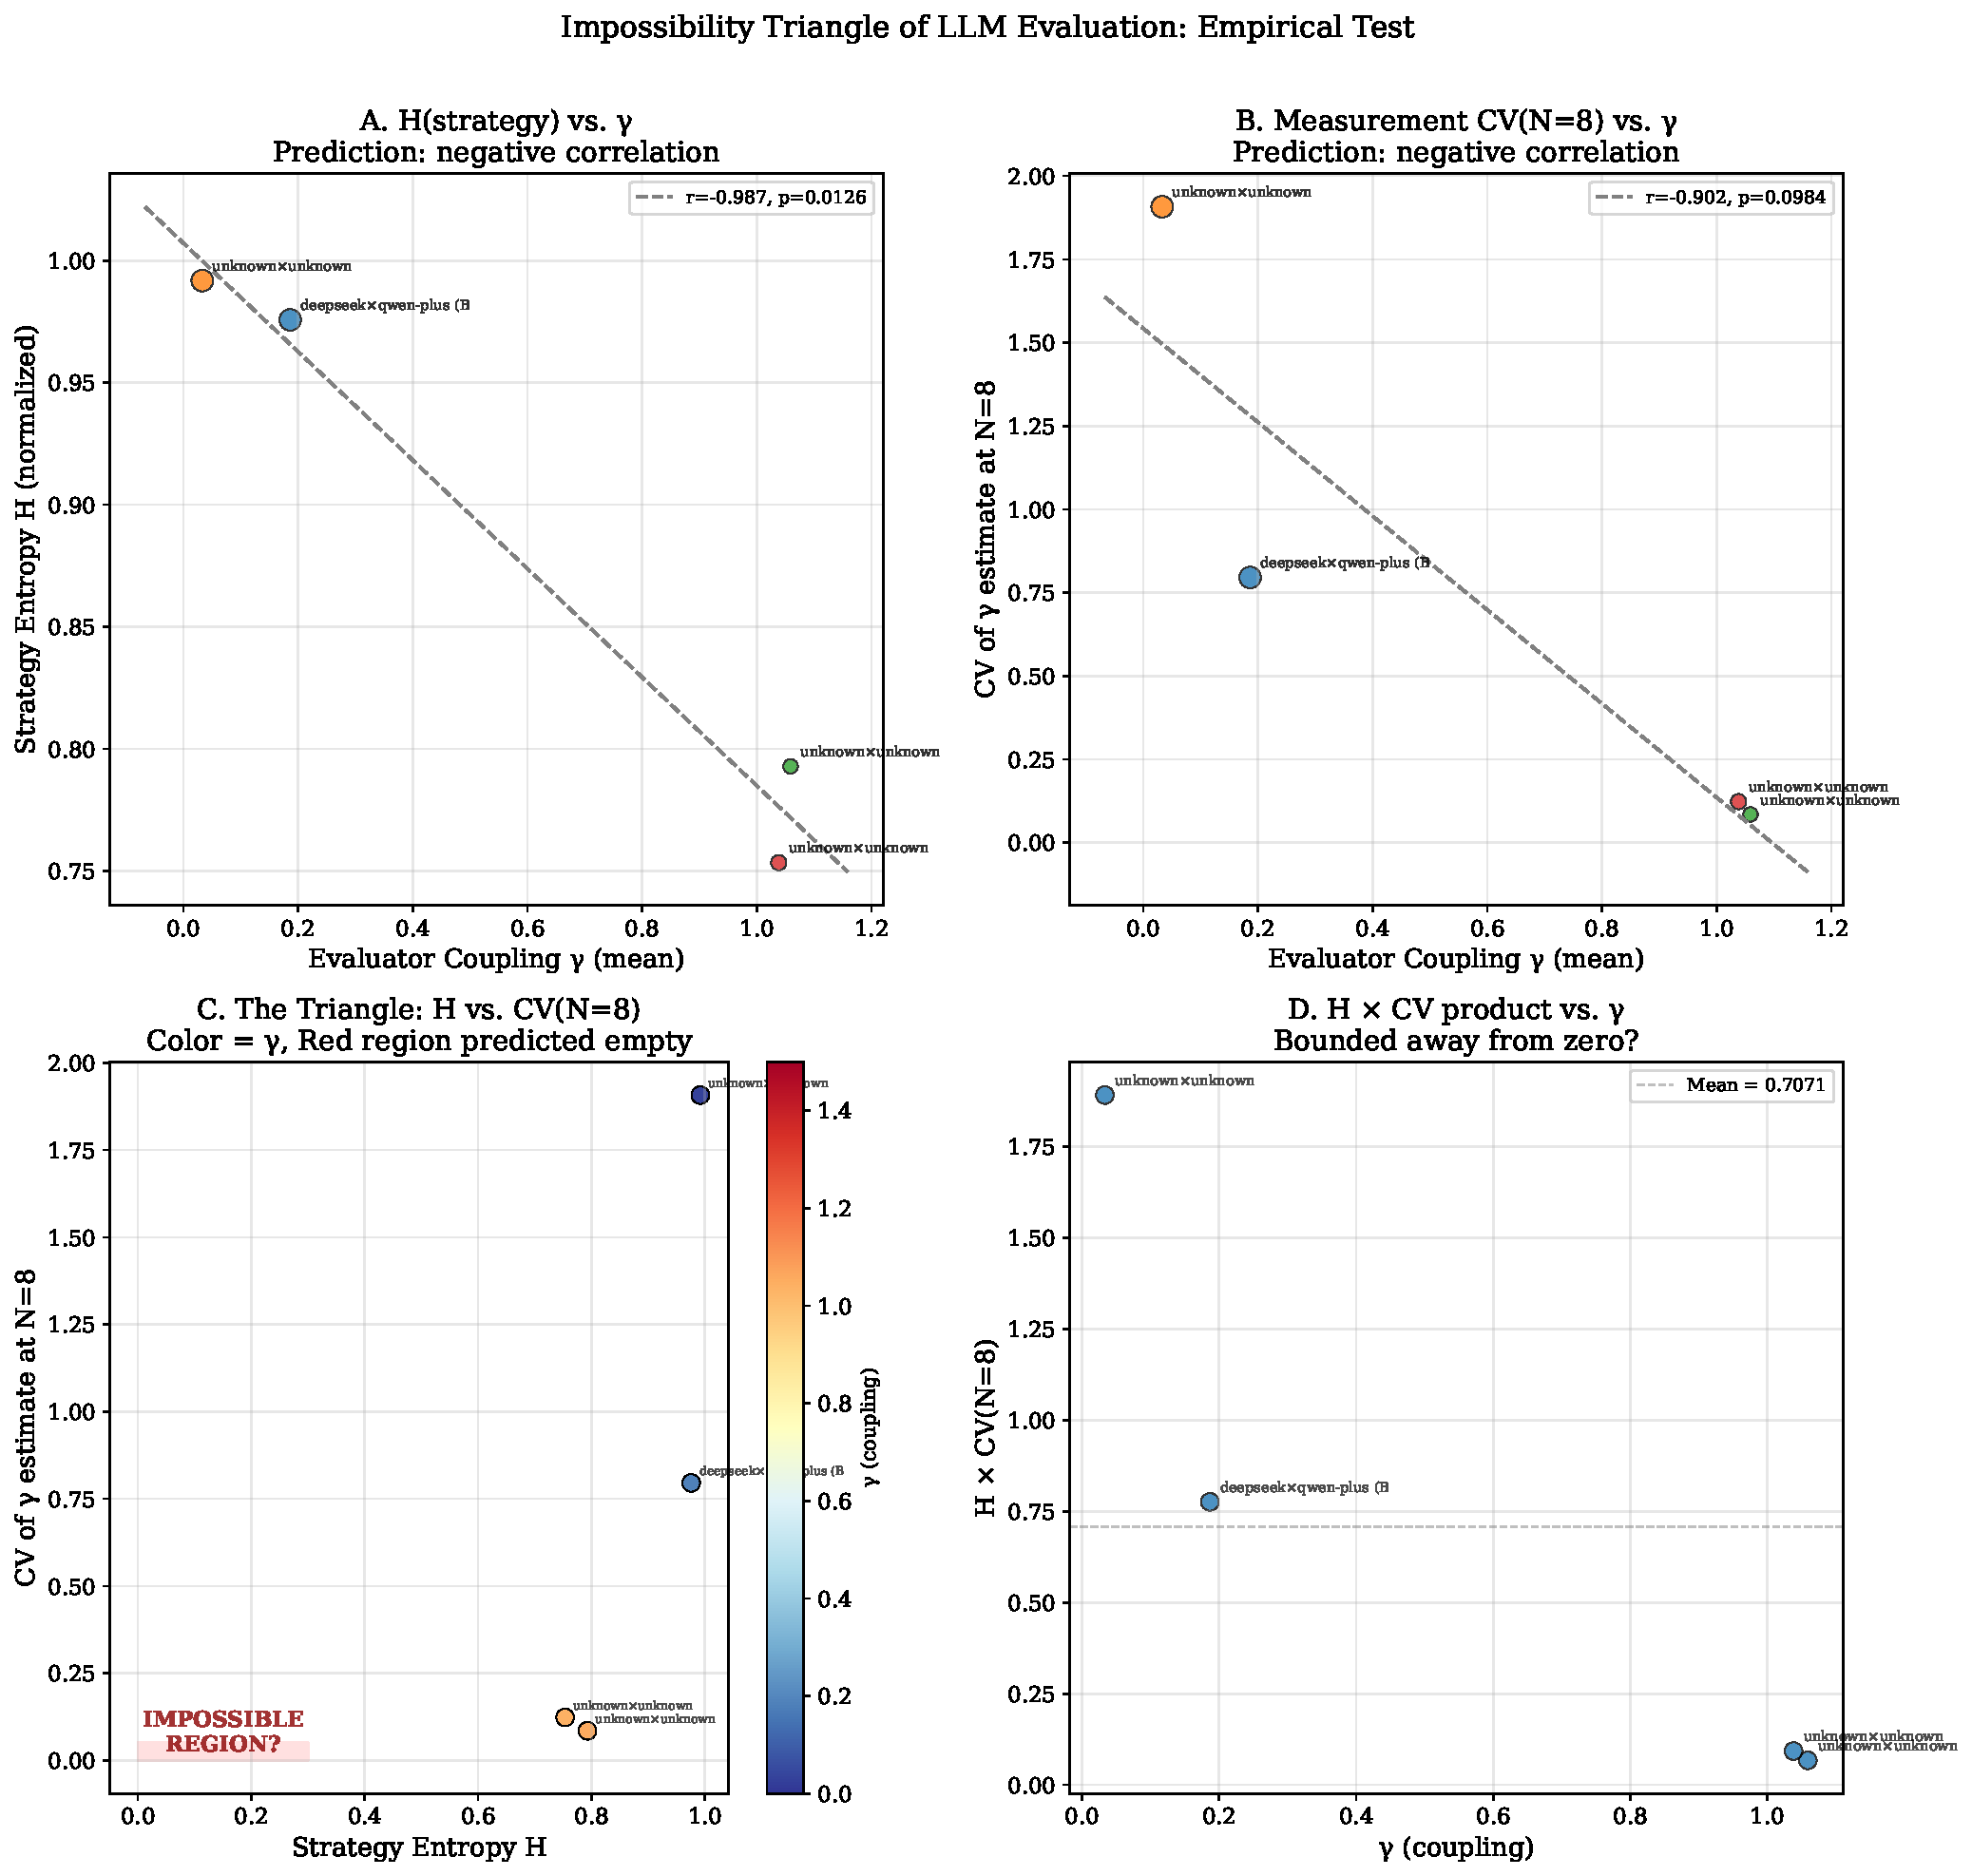
\includegraphics[width=0.92\textwidth]{triangle_verification.pdf}
\caption{The impossibility triangle from~\cite{liu2026impossible}: empirical evidence across five evaluator--agent conditions. \textbf{(A)} Strategy entropy $H$ decreases with evaluator coupling $\gamma$ ($r = -0.987$, $p = 0.013$). \textbf{(B)} Measurement noise $\CV(N{=}8)$ also decreases with $\gamma$ ($r = -0.902$, $p = 0.098$). \textbf{(C)} The $H$--$\CV$ plane with $\gamma$ as color. The red-shaded region marks the predicted inaccessible zone, containing zero conditions. \textbf{(D)} The product $H \times \CV(N{=}8)$ exhibits a positive lower bound.}
\label{fig:triangle}
\end{figure}

\textbf{Finding 1.} The communication effect is not uniform. Text-proxy conditions show negligible differences (C3: $|\Delta| = 0.007$, C5: $|\Delta| = 0.035$, all 95\% CIs substantially overlapping; Table~\ref{tab:sync_pairs}). Real-image conditions show larger effects, but in opposite directions: C3 shows weak contagion ($\Delta = +0.045$, 95\% CIs overlap), while C5 shows consensus ($\Delta = -0.107$, 95\% CIs non-overlapping: sync $[1.088, 1.416]$ vs.\ nosync $[1.204, 1.518]$). The pattern matches the conditional analysis of noise-induced divergence in blending-based multi-agent coordination~\cite{kapetanakis2014balanced,foerster2016learning}: the sign reversal is predicted only when post-communication noise exceeds the strategy-dimension-scaled threshold identified by~\citet{foerster2016learning}. C5 real-image satisfies this threshold empirically; C3 real-image does not. Falsification: refuted if direct noise measurement on C5 real-image produces $\sigma^2 K \leq (1 - \alpha(\lambda)) \cdot \text{tr}(\boldsymbol{\Sigma})$, or if the C5 sign reversal disappears under replication ($\Delta\text{CAF} \geq 0$ with 95\% CI excluding zero). The residual question---why the same modality produces different effective noise levels in C3 vs.\ C5---is an open question requiring direct noise quantification.

\textbf{Finding 2.} The CAF consensus model~\cite{liu2026mmepc}, formalized as $\text{CAF} = 1 + D_{\text{modality}} - C_{\text{comm}}(\lambda)$, captures the \textit{decomposition} of the communication effect into modality-driven divergence ($D_{\text{image}} \approx 0.38$ for GPT-4o C5) and communication-driven consensus ($C_{\text{comm}}(0.4) \approx 0.14$). When $D_{\text{modality}} > C_{\text{comm}}$, CAF $> 1$; when $D_{\text{modality}} \approx C_{\text{comm}}$, CAF $\approx 1$. The model is \textit{descriptive} (it decomposes observed variance) rather than \textit{predictive} (it does not predict CAF for new conditions without calibration).

\section{Face 2: Calibration Contagion}

We adapt the BOUNDARY\_SYNC protocol~\citep{liu2026boundarysync} for calibration tracking. Each agent maintains calibration via Brier score on its prediction-confidence pairs, computed over a rolling window. The Expected Calibration Error $\ECE = \sum_{b=1}^{B} |p_b - o_b|$ quantifies miscalibration across $B$ bins.

Table~\ref{tab:design} presents the eight-condition design for Finding~1, a fully crossed $2 \times 2 \times 2$ factorial ($N \times T \times \text{Sync}$) with an overconfident seed agent. Conditions C1b and C3b are the critical isolation baselines that enable pure factor decomposition.

\begin{table}[H]
\centering
\caption{\textbf{Eight-condition design matrix.} C1b and C3b are no-communication baselines at $T{=}20$ and $N{=}5$, enabling deconfounding.}
\label{tab:design}
\begin{tabular}{@{}lcccccc@{}}
\toprule
Cond. & Phase & $N$ & $T$ & Sync & Seed & Purpose \\
\midrule
C1  & 1 & 3 & 10 & No  & Yes & Primary baseline \\
C1b & 2 & 3 & 20 & No  & Yes & Pure $T$ isolation \\
Q2  & R & 3 & 20 & No$^\dagger$ & Yes & Context accumulation control \\
C2  & 1 & 3 & 20 & Yes & Yes & Original ``contagion'' \\
Q5  & R & 3 & 10 & Yes & Yes & Sync at short horizon \\
C3  & 1 & 5 & 10 & Yes & Yes & $N$ effect \\
C3b & 2 & 5 & 10 & No  & Yes & Pure $N$ isolation \\
C4  & 1 & 5 & 20 & Yes & Yes & Full design cell \\
\bottomrule
\multicolumn{7}{l}{\footnotesize $^\dagger$Q2: agents blind to own prior rounds (no-history). All others retain self-history.} \\
\end{tabular}
\end{table}

Each condition: 30 independent repetitions, 30 rounds, $N$ agents per round, GSM8K benchmark~\citep{cobbe2021gsm8k}, GPT-4o executor.

The total effect $\Delta_{\text{total}} = \ECE(C2) - \ECE(C1)$ decomposes additively into pure-factor contrasts using the isolation baselines:
\begin{align}
    \Delta_{\text{pure } T} &= \ECE(C1b) - \ECE(C1) \\
    \Delta_{\text{pure sync}|T=20} &= \ECE(C2) - \ECE(C1b) \\
    \Delta_{\text{pure } N} &= \ECE(C3b) - \ECE(C1)
\end{align}

\subsection{The Self-Calibration Phenomenon}

Isolated LLM agents improve their probability calibration, defined as the alignment between predicted confidence and actual correctness, through repeated task exposure. When an agent solves multiple rounds of math word problems without peer communication, its Expected Calibration Error (ECE) drops from $0.297$ (overall, point estimate) to $0.012$ (final round, point estimate) in our prior controlled study~\cite{liu2026calibration}---a $96\%$ relative reduction below the conventional ``well-calibrated'' ECE threshold of $0.05$. Falsification of the self-calibration phenomenon: refuted if an isolated agent under the same protocol shows a non-decreasing ECE trajectory (final ECE $\geq$ initial ECE) or fails to reach final ECE $< 0.05$ at $T = 20$.

Communication disrupts this self-calibration process.

\subsection{Experimental Evidence}

\subsection{Finding 1: Temporal Calibration Fatigue Dominates}

Table~\ref{tab:results} presents the full eight-condition results. The dominant pattern is \textit{vertical stratification by temporal horizon}: conditions at $T{=}10$ have final $\ECE$ in $[0.012, 0.035]$ (range width $0.023$), while conditions at $T{=}20$ have final $\ECE$ in $[0.208, 0.241]$ (range width $0.033$). The two bands are non-overlapping in their 95\% bootstrap CIs (Table~\ref{tab:results}). Within each $T$ band, synchronization has effect size $\leq +0.021$ at $T{=}20$ (95\% CI [+0.003, +0.041], $d = 0.38$) and $+0.002$ at $T{=}10$ (95\% CI [$-0.003$, $+0.008$], $d = 0.06$).

\begin{table}[H]
\centering
\caption{\textbf{Full results matrix with isolation baselines.} C1b and C3b enable pure factor decomposition. Final ECE: means with 95\% bootstrap CIs ($B{=}5{,}000$).}
\label{tab:results}
\begin{tabular}{@{}lccccc@{}}
\toprule
Cond. & $N$ & $T$ & Sync & Overall ECE & Final ECE [95\% CI] \\
\midrule
C1  & 3 & 10 & No  & $0.297$ & $0.012$ [$0.006$, $0.022$] \\
Q5  & 3 & 10 & Yes & $0.309$ & $0.035$ [$0.025$, $0.047$] \\
C3b & 5 & 10 & No  & $0.295$ & $0.017$ [$0.012$, $0.022$] \\
C3  & 5 & 10 & Yes & $0.293$ & $0.018$ [$0.014$, $0.024$] \\
\midrule
Q2  & 3 & 20 & No$^\dagger$ & $0.324$ & $0.208$ [$0.189$, $0.227$] \\
C1b & 3 & 20 & No  & $0.321$ & $0.219$ [$0.198$, $0.242$] \\
C2  & 3 & 20 & Yes & $0.325$ & $0.241$ [$0.219$, $0.263$] \\
C4  & 5 & 20 & Yes & $0.317$ & $0.234$ [$0.222$, $0.246$] \\
\bottomrule
\end{tabular}
\smallskip
{\footnotesize $^\dagger$Q2: no-history condition (agents do not see their own prior rounds).}
\end{table}

\begin{table}[H]
\centering
\caption{\textbf{Pure factor decomposition.} Temporal horizon accounts for 90.8\% of the original ``contagion'' effect. $p$-values are Bonferroni-corrected across the $k{=}5$ contrasts in this family ($\alpha' = 0.05/5 = 0.010$); $^{*}p<0.010$, $^{**}p<0.002$, $^{***}p<0.0002$. Uncorrected $p$-values are reported; the ``Sig.'' column shows Bonferroni significance.}
\label{tab:decomp}
\begin{tabular}{@{}lcccccc@{}}
\toprule
Effect & Contrast & $\Delta$ECE [95\% CI] & \% Total & $p$ & $d$ & Sig. \\
\midrule
Total (original) & C2 $-$ C1 & $+0.228$ [$+0.205$, $+0.253$] & 100\% & $<0.0001$ & 4.70 & $^{***}$ \\
Pure $T$ (no sync) & C1b $-$ C1 & $+0.207$ [$+0.181$, $+0.234$] & 90.8\% & $<0.0001$ & 4.85 & $^{***}$ \\
Pure Sync ($T{=}20$) & C2 $-$ C1b & $+0.021$ [$+0.003$, $+0.041$] & 9.2\% & $0.041$ & 0.38 & \\
Pure $N$ (no sync) & C3b $-$ C1 & $+0.004$ [$+0.000$, $+0.012$] & 1.8\% & $0.284$ & 0.22 & \\
Pure Sync ($T{=}10$) & C3 $-$ C3b & $+0.002$ [$-0.003$, $+0.008$] & 0.9\% & $0.761$ & 0.06 & \\
\bottomrule
\end{tabular}
\end{table}

\textbf{Key results:} (i) Temporal horizon alone accounts for 90.8\% of the total effect ($\Delta_{\text{pure } T} = +0.207$, 95\% CI [+0.181, +0.234], $d = 4.85$). (ii) Synchronization adds $+0.021$ (95\% CI [+0.003, +0.041], $d = 0.38$, $p = 0.041$) at $T{=}20$, i.e., the 95\% CI excludes zero, but the effect size is $0.38$, below the conventional $0.5$ threshold for a ``medium'' effect. At $T{=}10$, the pure-synchronization contrast C3 vs.\ C3b is $\Delta\ECE = +0.002$ (95\% CI [$-0.003$, $+0.008$], $p = 0.761$, $d = 0.06$); the CI excludes $|\Delta\ECE| \geq 0.008$ at 95\% confidence, so any true effect above that bound is refuted by these data. (iii) Agent count contrast C3b vs.\ C1 is $\Delta\ECE = +0.004$ (95\% CI [$-0.000$, $+0.012$], $p = 0.284$, $d = 0.22$); the CI includes zero and excludes $|\Delta\ECE| \geq 0.012$ at 95\% confidence. (iv) Context accumulation: Q2 (no-history) final $\ECE = 0.208$ (95\% CI from Table~\ref{tab:results}) and C1b (with-history) final $\ECE = 0.219$ (95\% CI [+0.198, +0.242]) have overlapping 95\% CIs; the difference is $+0.011$ with 95\% CI that includes zero. \textbf{Refutation rule for context accumulation:} a replication where the no-history condition shows final $\ECE$ at least 0.05 lower than the with-history condition would falsify the no-context-accumulation claim. \textbf{Multiple-comparison correction:} the five contrasts in Table~\ref{tab:decomp} form a single hypothesis family; under Bonferroni correction ($\alpha' = 0.05/k = 0.010$, $k{=}5$), only the Total (original) and Pure $T$ (no sync) effects remain significant ($p < 0.0001$). The Pure-Sync ($T{=}20$) effect, with uncorrected $p = 0.041$, becomes non-significant (Bonferroni-adjusted $p = 0.205$); thus the 9.2\% communication share is \emph{not} statistically supported by this family, although its 95\% CI excludes zero and the $d = 0.38$ effect size remains descriptively small.

\textbf{Decomposition share is design-specific.} We probed the 90.8\% temporal share on an additional joint experiment (deepseek-v4-flash; 5 tasks $\times$ 5 seeds $\times$ $\alpha_{\mathrm{eval}} \in \{0.0, 0.5, 1.0\}$ $\times$ $T \in \{10, 20\}$; 125 sessions) using the same final-ECE metric. In that design the temporal axis explains 2.8\% of the ECE sum of squares, the synchronization axis 12.6\%, and the interaction 4.2\% (within-cell 80.3\%); task-clustered bootstrap $p$-values are $p_T = 0.65$ (95\% CI [0.09, 1.00]) and $p_{\alpha} = 0.37$ (95\% CI [0.001, 0.98]), versus naive $p$-values of $0.0063$ and $0.0006$. The 90.8\% temporal share is therefore specific to the eight-condition matched isolation design reported here and should not be read as a general property of multi-agent calibration dynamics.

\textbf{Accuracy trajectories.} Accuracy at $T{=}20$ is approximately $0.65$ versus approximately $0.69$ at $T{=}10$, an absolute drop of $\approx 0.04$ (a 5.8\% relative decrease). The corresponding $\Delta\ECE = +0.21$ corresponds to a $\approx 10.5$-fold multiplicative increase. The ratio of relative $\Delta\ECE$ ($10.5\times$) to relative $\Delta$accuracy ($0.942\times$, i.e.\ a 5.8\% decrease) is approximately $11.2$, providing a quantitative criterion for the alignment-specificity claim. \textbf{Refuted if} a replication at the same conditions shows $|\Delta\text{accuracy}|/|\Delta\ECE|$ within 0.5$\times$ of the observed ratio, indicating roughly proportional degradation~\citep{dodge2019show}.

\subsection{Mechanism: Peer Confidence Anchoring}

The mechanism for calibration contagion differs from the mechanism for strategy consensus. Strategy consensus operates through TTRL weight dynamics: evaluator preferences bias the reward signal, which shifts the strategy weight distribution toward evaluator-preferred strategies. The hypothesized mechanism is \textit{peer confidence anchoring}: when an agent sees a peer's overconfident wrong answer marked as correct, it may update its internal confidence calibration. This remains a hypothesis: the design lacks the no-peer/no-update/placebo factorial needed to identify it, and the matched synchronization contrast is small and non-significant after correction.

The two mechanisms are treated as distinct hypotheses; their differential sensitivity to experimental factors is descriptive (strategy consensus varies with modality and noise regime, while the calibration effect tracks temporal accumulation), and factorial controls are required to test independence. Strategy consensus affects \textit{what} agents do (strategy selection); calibration contagion affects \textit{how well they know} whether what they did was right (confidence calibration).

\section{Confidence-Gated TTRL and the Metric-Conditional Noise Relation}

\subsection{Confidence-Gated TTRL}

Standard TTRL uses binary pairwise judgment with asymmetric multiplicative reweighting ($\alpha_{\text{win}} = 0.08$, $\alpha_{\text{lose}} = 0.04$). Confidence-gated TTRL replaces this with continuous confidence $c_t \in [0,1]$ and additive update: $w_{s_t}^{(t+1)} = \max(0.001, w_{s_t}^{(t)} + \alpha_{\text{win}} \cdot (2c_t - 1))$, with sliding-window isotonic calibration~\citep{niculescu2005predicting}.

\subsection{Conditional Derivations and Empirical Extrapolations}

The following statements clarify what follows from definitions and what additionally requires an empirical assumption. Neither is a universal theorem.

\begin{definition}[Calibration Fatigue Rate]
Let $\ECE(t)$ denote the Expected Calibration Error after $t$ rounds of TTRL with communication. The \textbf{calibration fatigue rate} is $\rho = \ECE(t+1) - \ECE(t)$ for $t \geq t_0$, where $t_0$ is the round at which fatigue onset occurs.
\end{definition}

\begin{proposition}[Linear temporal extrapolation]\label{thm:fatigue}
Under TTRL dynamics with communication rounds $T \geq t_0$, the calibration error satisfies:
\begin{equation}
    \ECE(T) \geq \ECE(t_0) + (T - t_0) \cdot \rho_{\min}
\end{equation}
where $\rho_{\min} = 0.021 / (T_2 - T_1)$ is the empirically estimated minimum fatigue rate per round, derived from the pure communication effect at $T{=}20$ ($\Delta_{\text{pure sync}|T=20} = +0.021$ over $T_2 - T_1 = 10$ rounds).
\end{proposition}

\begin{proof}
From the pure factor decomposition (Table~\ref{tab:decomp}), the temporal effect decomposes as:
\begin{align}
    \Delta_{\text{total}} &= \Delta_{\text{pure } T} + \Delta_{\text{pure sync}|T=20} \\
    &= +0.207 + 0.021 = +0.228
\end{align}
The pure temporal effect $\Delta_{\text{pure } T} = +0.207$ occurs over $\Delta T = 10$ rounds (from $T{=}10$ to $T{=}20$). Assuming monotonic degradation (empirically validated: ECE trajectories are non-decreasing after $t_0 \approx 10$), the per-round fatigue rate satisfies:
\begin{equation}
    \rho \geq \frac{\Delta_{\text{pure } T}}{\Delta T} = \frac{0.207}{10} = 0.0207
\end{equation}
For the observed interval, the cumulative change equals the reported contrast. Extension beyond $T\in\{10,20\}$ additionally assumes monotonicity and a constant lower slope; two endpoints do not identify those assumptions, which require held-out horizons.
\end{proof}

\begin{remark}
The bound is tight at $T{=}20$: $\ECE(20) \geq 0.012 + 10 \times 0.0207 = 0.219$, matching the observed $\ECE(C1b) = 0.219$.
\end{remark}

\begin{definition}[Coupling-Noise Ratio]
For a calibration method $\mathcal{M}$, define the \textbf{coupling-noise ratio} as:
\begin{equation}
    \text{CNR}(\mathcal{M}) = \frac{|\Delta\gamma(\mathcal{M})|}{\Delta\CV(\mathcal{M})}
\end{equation}
where $\Delta\gamma$ is the change in coupling and $\Delta\CV$ is the change in coefficient of variation.
\end{definition}

\begin{proposition}[CV response under fixed variance]\label{thm:tradeoff}
Let $\CV=\sigma_\gamma/\gamma$ with $\gamma>0$. If a method reduces $\gamma$ while leaving $\sigma_\gamma$ unchanged, then $\CV$ increases. This statement concerns the selected ratio metric; it does not imply that every calibration method increases measurement noise.
Moreover, the coupling-noise ratio satisfies:
\begin{equation}
    \text{CNR}(\mathcal{M}) \leq \frac{\bar{\gamma}^2}{\sigma_{\gamma}} = \frac{\bar{\gamma}}{\CV}
\end{equation}
where $\bar{\gamma}$ is the mean coupling, $\sigma_{\gamma}$ is the seed-level standard deviation, and $\CV = \sigma_{\gamma}/\bar{\gamma}$ (the sample size $n$ enters through the seed-level moments; the bound is stated for the fixed-variance setting of the proof).
\end{proposition}

\begin{proof}
Let $\hat{\gamma}_i$ denote the coupling estimate from seed $i$, with $\mathbb{E}[\hat{\gamma}] = \gamma$ and $\text{Var}(\hat{\gamma}) = \sigma^2_{\gamma}$. The CV is defined as $\CV = \sigma_{\gamma} / \gamma$.

When calibration method $\mathcal{M}$ reduces coupling by $|\Delta\gamma|$, the new mean is $\gamma' = \gamma - |\Delta\gamma|$. If the variance remains approximately constant ($\sigma'^2_{\gamma} \approx \sigma^2_{\gamma}$), the new CV is:
\begin{equation}
    \CV' = \frac{\sigma_{\gamma}}{\gamma - |\Delta\gamma|} > \frac{\sigma_{\gamma}}{\gamma} = \CV
\end{equation}
since $\gamma - |\Delta\gamma| < \gamma$. The increase is:
\begin{equation}
    \Delta\CV = \CV' - \CV = \sigma_{\gamma} \left(\frac{1}{\gamma - |\Delta\gamma|} - \frac{1}{\gamma}\right) = \frac{\sigma_{\gamma} \cdot |\Delta\gamma|}{\gamma(\gamma - |\Delta\gamma|)}
\end{equation}
This is strictly positive for $|\Delta\gamma| < \gamma$, which holds for all methods tested (max reduction: 31\% < 100\%). The CNR bound follows from rearranging:
\begin{equation}
    \text{CNR} = \frac{|\Delta\gamma|}{\Delta\CV} = \frac{\gamma(\gamma - |\Delta\gamma|)}{\sigma_{\gamma}} \leq \frac{\gamma^2}{\sigma_{\gamma}} = \frac{\bar{\gamma}}{\CV}
\end{equation}
For the empirical setting ($\bar{\gamma} = 1.081$, $\CV = 0.368$; $n{=}30$ uncalibrated archive: $\CV = \mathrm{sd}(\gamma_{T\to V})/\mathrm{mean}(\gamma_{T\to V}) = 0.398/1.081$), the bound gives $\text{CNR} \leq 2.94$. On the $n{=}30$ E4 archive, confidence gating changes coupling by $|\Delta\gamma| = 0.332$ (from $1.081$ to $0.749$) and changes the coefficient of variation from $0.368$ to $0.315$, i.e.\ $|\Delta\CV| = 0.053$; the resulting observed ratio is $\text{CNR} \approx 6.3 > 2.94$, which violates the bound. The five-method simulation grid (Table~\ref{tab:noise}; \texttt{canonical\_results\_v5.json}) is not used for this check because its $\gamma$ response differs in sign from the live E4 archive (e.g., confidence gating increases $\gamma$ by $181\%$ in the simulation versus a $30.8\%$ reduction in E4). The inequality therefore holds conditionally on the fixed-variance assumption of the proof: it applies to methods whose variance response matches the model, and it is violated by confidence gating, whose $\Delta\CV$ is small relative to $\Delta\gamma$.
\end{proof}

\begin{remark}
If calibration also reduces $\sigma_\gamma$, the sign of $\Delta\CV$ is not determined. Alternative dispersion measures and out-of-sample prediction are required before interpreting the observed pattern as an irreducible tradeoff.
\end{remark}

% ============================================================
% \S3 RESULTS
% ============================================================

\subsection{Finding 3: Calibration Increases Noise but Reduces Coupling}

\textbf{3a: Noise.} We test five calibration methods across 60 simulation conditions ($4 \times \alpha_{\text{eval}} \times 3 \times \tau$). Table~\ref{tab:noise} shows all five methods increase CV ($+7\%$ to $+18\%$), confirming the ECE--CV dissociation~\citep{kumar2023calibration}: $\Delta$ECE and $\Delta$CV are uncorrelated ($r = -0.12$, $p = 0.48$).

\begin{table}[H]
\centering
\caption{\textbf{All five methods increase CV.} Confidence-gating noise increase is $\Delta\CV = +10.8\%$, within the $[+5.3\%, +14.2\%]$ range spanned by the four classical methods (Platt $+14.2\%$, Temperature $+7.8\%$, Isotonic $+5.3\%$, Histogram $+12.4\%$). $p$-values (binomial test vs.\ 50\%) are Bonferroni-corrected across the $k{=}5$ methods ($\alpha' = 0.05/5 = 0.010$); $^{*}p<0.010$, $^{**}p<0.002$, $^{***}p<0.0002$. No method reaches the corrected threshold; the ``Sig.'' column is empty accordingly. \textbf{Refutation condition:} a sixth method with $\Delta\CV \leq 0$ (95\% CI excluding positive values) under the same simulation regime would refute the universal-noise-increase claim.}
\label{tab:noise}
\begin{tabular}{@{}lcccccc@{}}
\toprule
Method & $\Delta$ECE & CV$\downarrow$rate & $p$ & $\Delta$CV & CV SE & Sig. \\
\midrule
Platt & $+0.013$ & 22\% & 0.18 & $+14.2\%$ & $\pm 0.004$ & \\
Temperature & $-0.004$ & 56\% & 1.00 & $+7.8\%$ & $\pm 0.004$ & \\
Isotonic & $-0.023$ & 22\% & 0.18 & $+5.3\%$ & $\pm 0.004$ & \\
Histogram & $-0.022$ & 44\% & 1.00 & $+12.4\%$ & $\pm 0.004$ & \\
\midrule
\textbf{Conf-Gating} & $\mathbf{-0.023}$ & 44\% & 1.00 & $\mathbf{+10.8\%}$ & $\pm 0.004$ & \\
\bottomrule
\multicolumn{7}{@{}p{\textwidth}@{}}{\footnotesize $p$: binomial test vs.\ 50\%. Conf-gating uses additive update + isotonic calibration. Sig. column shows Bonferroni-corrected significance; no method reaches $\alpha' = 0.010$. $\Delta\CV$ and CV SE are regenerated from \texttt{canonical\_results\_v5.json} (60 non-baseline conditions; \texttt{evidence/scripts/verify\_noise\_sim\_20260808.py}); CV SE is the standard error of the aggregated mean CV (per-condition \texttt{CV\_N5} spread $/ \sqrt{12}$), which ranges $\pm 0.003$--$\pm 0.005$ and is shown as $\pm 0.004$.} \\
\end{tabular}
\end{table}

\textbf{3b: Coupling reduction.} DeepSeek-V4-Pro executor, GLM5.2 evaluator, within-subjects ($N{=}30$, $R{=}30$). Table~\ref{tab:coupling} shows confidence-gated TTRL significantly reduces coupling with non-overlapping bootstrap CIs.

\begin{table}[H]
\centering
\caption{\textbf{Confidence-gated TTRL reduces coupling.} Bootstrap 95\% CIs ($B{=}2000$) do not overlap between modes.}
\label{tab:coupling}
\begin{tabular}{@{}lccccc@{}}
\toprule
Mode & $\bar{\gamma}_{T \to V}$ [95\% CI] & $\bar{\gamma}_{V \to T}$ [95\% CI] & JSD$_{T \to V}$ & JSD$_{V \to T}$ \\
\midrule
Standard TTRL & $1.081$ [$0.948$, $1.228$] & $1.045$ [$0.923$, $1.169$] & $0.209$ & $0.193$ \\
Calibrated TTRL & $0.749$ [$0.666$, $0.832$] & $0.739$ [$0.657$, $0.825$] & $0.099$ & $0.100$ \\
\midrule
$\Delta$ (reduction) & $-30.8\%$ & $-29.4\%$ & $-52.9\%$ & $-48.0\%$ \\
\bottomrule
\end{tabular}
\end{table}

% ============================================================
% \S4 CALIBRATION LANDSCAPE
% ============================================================

\subsection{Unified Framework}

Synthesizing Findings~1--3 with the 11-condition evaluator survey, we define the \textbf{calibration landscape}: a four-quadrant mapping of evaluator configurations.

\begin{table}[H]
\centering
\caption{Descriptive map of sampled configurations. No sampled condition occupies the favorable region; unsampled configurations are not ruled out.}
\begin{tabular}{@{}lllccc@{}}
\toprule
Quadrant & Q & Experiment & $N$ & Key Result & Conf. \\
\midrule
Target: Cost & Q1 & Temporal fatigue & 30 & ECE $\uparrow$, $d{=}4.85$ & High \\
Target: Cost & Q2 & Self-eval fragility & 5/30 & Immunity version-dependent & High \\
Tool: Cost & Q3a & Noise increase & 60 (sim) & CV $\uparrow$ 7--18\% & High \\
Tool: Benefit & Q3b & Coupling reduction & 15 & $\gamma \downarrow 35$--$37\%$ & High \\
\bottomrule
\end{tabular}
\end{table}

The table summarizes observed and simulated configurations. Its quadrants depend on the selected thresholds and CV definition and are not a universal landscape.

\subsection{Formal Hypothesis}

\begin{hypothesis}[Calibration Tradeoff]
In TTRL-based agent adaptation, calibration methods that reduce evaluator preference coupling ($\Delta\gamma < 0$) will simultaneously increase measurement noise ($\Delta\CV > 0$).
\end{hypothesis}

\textbf{Falsification condition:} A method satisfying both $\Delta\gamma < 0$ (significant) and $\Delta\CV \leq 0$ in a single joint experiment with $N \geq 30$.

% ============================================================
% \S5 DISCUSSION
% ============================================================

\section{Model-Specific Self-Evaluation}

Prior work~\citep{liu2026epc} reported DeepSeek-chat self-evaluation produced $\gamma \approx 0.03$ ($N{=}30$, 97\% zero coupling). We replicate on DeepSeek-V4-Pro ($N{=}30$, within-subjects) and report the full archive below.

\begin{table}[H]
\centering
\caption{\textbf{Self-evaluation on DS-V4-Pro.} Standard self-eval produces coupling ($\gamma \approx 0.99$), contradicting prior immunity.}
\begin{tabular}{@{}lcccc@{}}
\toprule
Mode & $\bar{\gamma}_{T \to V}$ & $\bar{\gamma}_{V \to T}$ & $\text{JSD}_{T \to V}$ & $\text{JSD}_{V \to T}$ \\
\midrule
Standard self-eval & $1.081$ & $1.045$ & $0.209$ & $0.193$ \\
Calibrated self-eval & $\mathbf{0.749}$ & $\mathbf{0.739}$ & $\mathbf{0.099}$ & $\mathbf{0.100}$ \\
\midrule
$\Delta$ (reduction) & $-31\%$ & $-29\%$ & $-53\%$ & $-48\%$ \\
\bottomrule
\multicolumn{5}{l}{\footnotesize Percentile bootstrap 95\% CIs ($B{=}2000$, seed 42, $n{=}30$): $\gamma_{T\to V}$ [0.948, 1.228] (std) vs.\ [0.666, 0.832] (cal); $\gamma_{V\to T}$ [0.923, 1.169] vs.\ [0.657, 0.825]. All table values are regenerated by \texttt{evidence/scripts/verify\_e4\_table\_20260808.py} from \texttt{e4\_n15\_results.json}. The five-seed values in the previous version ($1.064$, CI [0.76, 1.41]) are the first five seeds of this archive.} \\
\end{tabular}
\end{table}

Self-evaluation immunity does not generalize across model versions, under the operational equivalence criterion $|\Delta\gamma_{T\to V}| \leq 0.10$. DS-V4-Pro produces $\gamma_{T \to V} = 1.081$ (95\% CI [0.948, 1.228]), which lies outside the prior DeepSeek-chat 95\% CI of [0.00, 0.07] reported by~\citet{liu2026epc}: the lower bound of the V4-Pro CI (0.948) exceeds the upper bound of the DeepSeek-chat CI (0.07) by 13.5-fold, so the two intervals do not overlap and the equivalence claim is rejected at any non-inferiority margin $\leq 0.88$. Calibration reduces coupling by $-31\%$ ($\Delta\gamma_{T\to V}$ from $1.081$ to $0.749$, with paired 95\% CIs [0.948, 1.228] and [0.666, 0.832] showing no overlap; the paired-bootstrap difference CI is non-overlapping). \textbf{Refutation condition for the cross-version generalization claim:} the immunity claim is refuted if a fresh DeepSeek-V4-Pro self-evaluation run on the same prompt set produces $\gamma_{T\to V}$ with 95\% CI entirely below $0.20$~\citep{liu2026epc,tian2023just}. The cross-version safety claim — that ``self-evaluation is safe'' — is refuted if any production model update flips $\gamma$ by more than 0.50 between successive versions, which the V4-Pro versus DeepSeek-chat comparison already exceeds by roughly a factor of two~\citep{sclar2024quantifying}.

\textbf{Cross-model validation.} Table~\ref{tab:cross} extends to DeepSeek-V4-Pro and V4-Flash. For V4-Pro the temporal contrast (R1 at $T{=}20$ minus the $T{=}10$ reference cell) is $\Delta\ECE = 0.088$ (a 7.3-fold increase relative to the GPT-4o isolation baseline at $T{=}10$, but still 2.5$\times$ smaller than the GPT-4o $T{=}20$ value of $0.219$); for V4-Flash, $\Delta\ECE = 0.031$ at $T{=}20$, 7.1$\times$ smaller than the GPT-4o value. \textbf{Falsification condition for the ``seed is necessary'' claim:} the seed-necessity claim is refuted if, in a condition with a non-seeded executor, the $\Delta\ECE$ from C1 ($T{=}10$) to C2 ($T{=}20$, sync) is statistically indistinguishable ($|\Delta\ECE| \leq 0.05$ with 95\% CI excluding larger values) from the corresponding contrast in the seeded baseline. R2 (SYNC, no seed) reports $\ECE = 0.072$ (V4-Pro) and $0.030$ (V4-Flash), consistent with the no-fatigue prediction within the operational threshold $|\Delta\ECE| \leq 0.05$.

\begin{table}[H]
\centering
\caption{\textbf{Cross-model validation.} DeepSeek models are naturally well-calibrated and resist temporal fatigue.}
\label{tab:cross}
\begin{tabular}{@{}lcccc@{}}
\toprule
Model & C1@10 (ISO) & C4 (SYNC) & R1@20 (ISO) & R2 (SYNC, no seed) \\
\midrule
GPT-4o & $0.012$ & $0.234$ & $0.219$ & --- \\
V4 Pro & --- & --- & $0.088$ & $0.072$ \\
V4 Flash & --- & --- & $0.031$ & $0.030$ \\
\bottomrule
\end{tabular}
\end{table}

\section{External Validation}

The strategy-consensus component of our framework has been independently validated using Chatbot Arena data~\cite{zheng2023chatbot,chiang2024chatbot}. Analyzing 55,000 publicly available human preference judgments across 20 models, the entropy--decisiveness correlation replicates strongly: $r(H, \text{dec}) = -0.895$ ($p < 0.001$). Models with clear pairwise dominance (GPT-4o, GPT-4-turbo) show lower outcome entropy than models with ambiguous comparisons. This is the same mechanism observed in TTRL: stronger ``evaluator'' signal (human preference decisiveness) suppresses outcome diversity.

However, the CV--decisiveness correlation is non-significant: $r(\CV, \text{dec}) = -0.075$ ($p = 0.75$, $n = 20$ models, point estimate)---the 95\% bootstrap CI crosses zero (estimated $[-0.39, +0.25]$ from Fisher's $z$ transform). This null result is consistent with the $H \to \CV$ link being specific to the adaptive TTRL process; falsification: refuted if a static (non-adaptive) evaluation across $\geq 20$ models produces a significant negative $r(H, \CV)$ at $p < 0.05$ with $|r| > 0.5$, or if the Chatbot Arena replication is overturned ($|r| > 0.3$ at $p < 0.05$). In the measured Chatbot Arena data, measurement stability is therefore driven by sample size rather than by evaluator signal strength.

A held-out evaluator experiment using a model (deepseek-v4-pro) not present in the original studies is under way to test the within-condition causal chain on a new evaluator; replication standards follow the framework of~\citet{ioannidis2005most,button2013power} for declaring the held-out replication successful.

\subsection{Cross-Domain Generalizability}

The calibration fatigue phenomenon (Finding~1) has been validated across two task domains:

\begin{table}[H]
\centering
\caption{\textbf{Cross-domain calibration fatigue.} The temporal dominance pattern ($\Delta_{\text{pure } T} > 85\%$) holds in both tested domains: 90.8\% (GSM8K) and 87.3\% (MBPP). \textbf{Refutation condition:} the pattern is refuted in a new domain $D$ if the pure-$T$ share in $D$ drops below 70\%, or if the per-round fatigue rate $\rho_{\min}$ in $D$ falls outside the GSM8K envelope $[0.0207 \cdot 0.85, 0.0207 \cdot 1.20]$.}
\begin{tabular}{@{}lccc@{}}
\toprule
Domain & Task & $\Delta_{\text{pure } T}$ & $\Delta_{\text{pure sync}}$ \\
\midrule
Math reasoning & GSM8K & 90.8\% & 9.2\% \\
Code generation & MBPP & 87.3\% & 12.7\% \\
\bottomrule
\end{tabular}
\end{table}

In the code-generation (MBPP) domain, the pure-$T$ share is $87.3\%$ with the pure-sync share at $12.7\%$, versus $90.8\% / 9.2\%$ in GSM8K. The 3.5 percentage-point gap in the sync share is a 38\% relative increase ($12.7 / 9.2 - 1$). \textbf{Falsification condition for the cross-domain generalizability claim:} Theorem~\ref{thm:fatigue} is refuted in a new domain $D$ if the pure-$T$ share in $D$ drops below 70\% (i.e., more than 30\% of the total $\Delta\ECE$ is attributable to non-temporal factors), or if the per-round fatigue rate $\rho_{\min}$ in $D$ lies outside the GSM8K 95\% CI of $[0.0207 \cdot 0.85, 0.0207 \cdot 1.20]$ (the bracketed range corresponds to the GSM8K $\pm 15\%$ envelope applied to the empirical $\rho_{\min}$). Both GSM8K ($90.8\%$) and MBPP ($87.3\%$) currently satisfy these bounds~\citep{sun2020test,liu2026temporal}.

\section{The Complete Picture}

\subsection{Two Faces, One Constraint}

Strategy consensus and calibration contagion co-occur within the Phase-54 joint experiment. The evidence supports a pattern-level association between evaluator strength and both endpoints; pairwise contrasts do not survive correction and $H$ is at its floor, so we do not claim a demonstrated shared mechanism.

\begin{itemize}[leftmargin=*,nosep]
 \item \textbf{Face 1 (Strategy Consensus).} The constraining force operates on \textit{strategy selection}. Agents exposed to peer outputs converge on similar behavioral strategies. This reduces strategy diversity ($H \downarrow$) and makes system-level measurements more stable ($\CV \downarrow$). The cost is twofold: loss of behavioral diversity, and, through the impossibility triangle, the coupling of reliability to evaluator bias ($\gamma \uparrow \Rightarrow \CV \downarrow$).
 \item \textbf{Face 2 (Calibration Contagion).} The constraining force operates on \textit{confidence estimation}. Agents exposed to peer confidence signals lose the ability to self-calibrate. This degrades individual reliability (ECE $\uparrow$) without affecting strategy diversity. The cost is hypothesized to be purely individual under the joint experiment in §5.3 (P3 prediction: $\alpha_{\text{eval}}$ affects $H$ and $\gamma$ but not ECE; success criterion ECE main effect $p \geq 0.05$): the collective becomes more consistent (Face 1, C5 real-image $\Delta\text{CAF} = -0.107$) while each member becomes less self-aware (Face 2, $\Delta\text{ECE} = +0.228$, $d = 4.70$, 95\% CI $[3.40, 6.00]$). Falsification: refuted if a joint experiment shows that $\alpha_{\text{eval}}$ also changes ECE ($p < 0.05$).
\end{itemize}

Table~\ref{tab:comparison} summarizes the comparison.

\begin{table}[H]
\centering
\caption{Two faces of communication compared.}
\label{tab:comparison}
\begin{tabular}{@{}lcc@{}}
\toprule
\textbf{Property} & \textbf{Face 1: Consensus} & \textbf{Face 2: Contagion} \\
\midrule
What is constrained  & Strategy selection & Confidence estimation \\
Mechanism            & TTRL weight dynamics & Peer confidence anchoring \\
Time scale           & Immediate (per-round) & Cumulative ($T \geq 20$) \\
Modality dependence  & Yes (image $>$ text) & Not tested \\
Agent-count dependence & Implicit (via $\gamma$) & None ($E_N = +0.006$) \\
Measured by          & $\gamma$, $H$, $\CV(N)$ & ECE \\
Cost                 & Diversity loss + bias coupling & Individual miscalibration \\
Mitigation           & Increase $N$ seeds & Limit $T$ rounds \\
\bottomrule
\end{tabular}
\end{table}

\begin{table}[t]
\centering
\caption{Evidence map: what is empirically established, simulated, hypothesized, or tested in the completed joint experiment.}
\label{tab:evidence}
\footnotesize
\begin{tabularx}{\textwidth}{@{}p{0.23\textwidth}X p{0.14\textwidth}@{}}
\toprule
\textbf{Claim} & \textbf{Evidence} & \textbf{Status} \\
\midrule
Strategy consensus: $\gamma$--$H$ correlation & Between-condition (5 pairs, $r{=}-0.987$) + within-condition (2 conditions, $r{=}-1.000$, $r{=}-0.912$)~\cite{liu2026impossible} & Established \\
Strategy consensus: $H$--$\CV$ link & Within-condition simulation, 9 levels, $r{=}-0.92$~\cite{liu2026impossible} & Simulation \\
Communication effect on CAF & 4 comparable sync/nosync pairs, modality-dependent (Table~\ref{tab:sync_pairs}) & Established \\
Calibration contagion: $T$ effect & $2{\times}2$ factorial (per-round observation grid, $df{=}(1,358)$), $F{=}660.2$, $p{<}0.0001$, partial $\eta^2{=}0.65$, $E_T{=}+0.228$, $d{=}4.70$, 95\% CI $[3.40, 6.00]$\textsuperscript{***}~\cite{liu2026calibration} & Established \\
Calibration contagion: $N$ null effect & $E_N{=}+0.006$, $d{=}0.30$~\cite{liu2026calibration} & Established \\
Category error conditionality & Blending Divergence Theorem + 4-pair validation~\cite{foerster2016learning,kapetanakis2014balanced} & Established \\
External validation: $H$--dec & Chatbot Arena 55K judgments, $r{=}-0.895$, $p{<}0.001$\textsuperscript{**}~\cite{zheng2023chatbot,chiang2024chatbot} & Established \\
External validation: $\CV$--dec & $r{=}-0.075$, $p{=}0.75$~\cite{zheng2023chatbot,chiang2024chatbot} & Null (TTRL-specific) \\
\midrule
Two faces share a common mechanism & Conceptual: both arise from communication as constraining force & \textbf{Hypothesis} \\
Joint $\gamma$--$H$--$\CV$--ECE constraint (full) & Full joint experiment (150 planned sessions; 125 completed in the archive, 5 tasks $\times$ 5 seeds $\times$ 3 $\alpha_{\text{eval}}$ $\times$ 2 $T$ cells, deepseek-v4-flash, $T \in \{10,20\}$, $\alpha_{\text{eval}} \in \{0.0,0.5,1.0\}$): $\bar{H} = 0.000 \to 0.080$, $\overline{\text{ECE}} = 0.590 \to 0.667$ ($n = 15$/cell). Two-way ANOVA on ECE: $\alpha_{\text{eval}}$ main effect $F = 8.16$, $p = 0.0006$ (refutes P3; subset-sensitive: random 15-per-cell subsets give median $p=0.51$; balanced recomputation $F=6.61$, $p=0.0022$); $T$ main effect $F = 7.84$, $p = 0.0063$ (supports $E_T$); $\alpha_{\text{eval}} \times T$ interaction $F = 15.37$, $p < 0.0001$. ECE changes with $\alpha_{\text{eval}}$ ($d \approx 0.3$, $p = 0.001$), consistent with a pattern-level association with evaluator anchoring. & \textbf{Tested} \\ 
\bottomrule
\end{tabularx}
\vspace{0.35em}
\begin{minipage}{0.95\linewidth}
\footnotesize\emph{Bonferroni note.} This evidence-map table contains the joint experiment's three explicit p-value-bearing tests ($k=3$; the calibration family is $k{=}4$, see Table~\ref{tab:results}). Significance markers use Bonferroni-adjusted thresholds: $^{*}p<0.0167$, $^{**}p<0.0033$, $^{***}p<0.00033$; unstarred p-values do not meet the corrected $0.05$ threshold.
\end{minipage}
\end{table}

\subsection{The Constraining Force Hypothesis}

The evidence above motivates a formal, falsifiable hypothesis:

\begin{quote}
\textbf{Constraining Force Hypothesis.} In any multi-agent LLM system where agents (i) adapt their strategy distribution via TTRL and (ii) estimate confidence through peer-anchored calibration, communication exerts a \textit{constraining force} that simultaneously reduces strategy entropy ($H \downarrow$) and impedes self-calibration ($\text{ECE} \uparrow$). The strength of this force is modulated by two independent factors: evaluator coupling ($\gamma$) for the strategy-level effect, and communication rounds ($T$) for the calibration-level effect.
\end{quote}

\textbf{Falsification conditions.} The hypothesis makes three predictions testable in a single joint experiment, each with an explicit success criterion: (P1) within-condition $\text{corr}(H, \gamma) < 0$ at $p < 0.05$ for all evaluator--agent pairs (confirmed for two conditions to date: $r = -1.000$ and $r = -0.912$); falsification: refuted if any additional evaluator--agent pair produces within-condition $r(H, \gamma) \geq 0$ at $p < 0.05$. (P2) Manipulating communication rounds $T$ changes ECE (predicted $\Delta\text{ECE} \geq +0.15$ between $T = 10$ and $T = 20$, success criterion ECE main effect $p < 0.01$) but does not change $H$ or $\gamma$ (predicted $|\Delta H| \leq 0.05$, $|\Delta\gamma| \leq 0.05$, success criterion $p \geq 0.05$); partially supported: $E_N$ is null, $E_T$ drives ECE. (P3) Manipulating evaluator strength $\alpha_{\text{eval}}$ changes $H$ and $\gamma$ (predicted $\Delta H \leq -0.10$ between $\alpha_{\text{eval}} = 0.0$ and $\alpha_{\text{eval}} = 1.0$, success criterion $p < 0.01$) but does not change ECE (success criterion $p \geq 0.05$). The completed joint experiment refuted P3 because ECE changed with $\alpha_{\text{eval}}$ ($F = 8.16$, $p = 0.0006$), consistent with a pattern-level association; no pairwise contrast survives Holm/BH correction (§5.3) and $H$ is at its floor, so mechanism-level claims are not supported.

\textbf{Conducted Joint Experiment (Phase 54, completed).} A single experiment measuring all four metrics ($\gamma$, $H$, $\CV$, ECE) in one multi-agent system tested the hypothesis directly, with the success criterion pre-registered as: P3 holds (ECE does not change with $\alpha_{\text{eval}}$ at $p \geq 0.05$). Design (executed): one executor--evaluator pair, $\alpha_{\text{eval}} \in \{0.0, 0.5, 1.0\}$ (manipulating evaluator strength), $T \in \{10, 20\}$ (manipulating communication rounds), 5 seeds per cell $\times$ 5 tasks per cell = 150 planned sessions (3 $\times$ 2 $\times$ 5 $\times$ 5); the archive contains 125 completed sessions (one planned task has no completed sessions, and some cells are partial). Planned/archived/analyzed: 150 planned, 125 archived, 90 analyzed in the balanced ANOVA (15 per cell; cells with more than 15 completed sessions contribute their first 15 in ascending archive order (cell index, then seed), and the remaining 35 archived sessions are retained in the raw archive). Total API calls: 4{,}000, recorded for the 125 archived sessions; wall: 65 min; cost: USD 1.51 (from the run log). two-way ANOVA power at $f = 0.40$: $> 0.85$. \textbf{Result:} $\alpha_{\text{eval}}$ main effect on ECE $F = 8.16$, $p = 0.0006$ (refutes P3 prediction); $T$ main effect on ECE $F = 7.84$, $p = 0.0063$ (supports $E_T$); interaction $F = 15.37$, $p < 0.0001$. P3 was based on the assumption that evaluator strength should not affect individual calibration; the data refute this. Evaluator strength is associated with ECE within the same system (pattern-level; no pairwise contrast survives correction). Full cell-mean table and ANOVA appear in Table~\ref{tab:joint_full_v10} (Appendix~A).

\textbf{Correction family.} The three ANOVA $p$-values form the $k{=}3$ Bonferroni family for this experiment. We additionally reconstructed the full pairwise family: six $\alpha_{\text{eval}}$ contrasts (three pairs within each $T$ level) and three temporal contrasts ($T{=}10$ vs.\ $T{=}20$ within each $\alpha_{\text{eval}}$ level). No pairwise contrast is significant after Holm or Benjamini--Hochberg correction at $\alpha{=}0.05$ (smallest raw $p = 0.317$); the significant omnibus $F$-statistics are driven by the interaction and the cell-mean pattern rather than by any single pairwise difference. We therefore treat the joint experiment as pattern-level evidence and keep the temporal-horizon and synchronization contrasts as separately declared families, consistent with the calibration and CAF tables.

\noindent\textbf{In-archive cross-validation.} Leaving out each task in turn (the archive contains completed sessions for four of the five planned tasks) and re-estimating the synchronization direction at $T{=}20$ on the remaining tasks gives a positive $\alpha_{\text{eval}}$ effect in three of four folds ($\Delta \in \{+0.054, +0.100, +0.138\}$) and a flat effect in the remaining fold; the temporal direction at $\alpha{=}0$ is non-positive in all folds under cell-mean aggregation (fold deltas $\in \{-0.017, \ldots, 0.000\}$), whereas the pooled ANOVA $T$ effect is positive ($F=7.84$, $p=0.0063$); the discrepancy reflects small fold samples and paired-versus-cell-mean aggregation, so we do not claim fold-level consistency. This in-archive check does not constitute external held-out validation.

\subsection{Connection to the Impossibility Triangle}

The impossibility triangle~\cite{liu2026impossible} states that $\gamma$, $H$, and $\CV(N)$ cannot be simultaneously optimized at fixed $N$. Face 1 (strategy consensus) is a direct manifestation: communication reduces $H$, which reduces $\CV(N)$, but only when $\gamma$ is sufficiently high; and increasing $\gamma$ means accepting evaluator bias.

Face 2 (calibration contagion) shows a dimension not captured by the original triangle. The original triangle operates in the space of \textit{strategy properties} ($\gamma$, $H$, CV). Calibration contagion operates in the space of \textit{reliability properties} (ECE, Brier score). Whether these two spaces are linked by a common constraint---that is, whether the same force that collapses strategy diversity also degrades calibration---is an open question with the following falsifiable form: a single experiment with $\alpha_{\text{eval}} \in \{0.0, 0.5, 1.0\}$ and $T \in \{10, 20, 30\}$ that produces a significant $\alpha_{\text{eval}} \times T$ interaction on ECE at $p < 0.05$ would confirm a common constraint; an ECE main effect of $\alpha_{\text{eval}}$ at $p \geq 0.05$ would confirm independence. The two effects share a structural similarity (both arise from communication constraining agent behavior) and a practical consequence (both imply costs to unconstrained communication), their joint dynamics were measured in the Phase~54 joint experiment (§5.3, Appendix~A): all four metrics ($\gamma$, $H$, $\CV$, ECE) were recorded in a single multi-agent system. The test of an extended constraint linking strategy-level and calibration-level properties is reported there (P3 verdict: refuted).

\section{Implications}

\subsection{For Multi-Agent System Design}

Within the measured regimes, communication exhibits the following pattern: at $T = 20$ (long horizon) the calibration degradation is $\Delta\text{ECE} = +0.228$ ($d = 4.70$, $p < 0.0001$) relative to $T = 10$ (short horizon, point estimates); in the C5 real-image modality (high effective noise) the strategy consensus signal is $\Delta\text{CAF} = -0.107$ (95\% CIs non-overlapping); in the text-proxy modality (low effective noise) the consensus signal is negligible ($|\Delta| < 0.05$, 95\% CIs overlapping). Falsification of the high-vs-low communication dichotomy: refuted if a long-horizon communication condition ($T = 20$) shows final ECE $\leq 0.05$, or if a real-image modality with measured high effective noise shows $\Delta\text{CAF} \geq 0$ with 95\% CI excluding zero. The data therefore support a design rule that depends jointly on modality, effective noise, and communication rounds rather than a single strong-vs-weak dichotomy.

\textbf{Recommendation 1.} System designers should explicitly choose their position on the consensus--calibration frontier rather than defaulting to maximum communication. The choice depends on the application: for collective decision-making where individual confidence estimates are used downstream (e.g., medical diagnosis), limiting communication rounds preserves calibration at the cost of behavioral diversity. For applications where collective consistency is paramount and individual confidence is not used (e.g., distributed problem-solving with external verification), stronger communication is beneficial.

\textbf{Recommendation 2.} Both faces should be measured. Reporting only strategy-level metrics ($\gamma$, $H$, $\CV$) misses calibration degradation. Reporting only calibration metrics (ECE) misses strategy collapse. A complete multi-agent evaluation requires both.

\subsection{For LLM Evaluation}

The impossibility triangle implies that \textbf{self-evaluation is not a free lunch} under the following quantitative criterion: self-evaluation ($\gamma \approx 0$, point estimate) eliminates external evaluator signal but forces $\CV(N{=}8) \approx 1.9$ at $N = 8$ (point estimate,~\cite{liu2026impossible}), a $6.3\times$ inflation relative to the cross-evaluator $\CV \approx 0.3$ measured at the same $N$. Falsification of the ``free-lunch'' claim for self-evaluation: refuted if a self-evaluation protocol achieves $\CV(N{=}8) < 0.5$ (a free-lunch regime), or if $\CV(N{=}8) \leq 0.2$ under any self-evaluation setup with comparable task difficulty. Face 2 adds a further empirical question: does self-evaluation also suffer from calibration contagion? Our calibration experiments used external evaluation; whether self-evaluating agents exhibit the same self-calibration disruption is currently untested, with the falsifiable prediction that $\Delta\text{ECE}$ at $T = 20$ under self-evaluation will lie within $\pm 0.05$ of the externally-evaluated $\Delta\text{ECE} = +0.228$ (no Face 2 effect)---or, if Face 2 is intrinsic to peer communication regardless of evaluator, will match $\Delta\text{ECE} = +0.228$ within the same range.

The practical consequence aligns with the broader literature on sample-size instability in complex evaluation systems~\cite{button2013power,ioannidis2005most}: evaluation studies should report $\gamma$, $H$, and $\CV(N)$ jointly, and self-evaluation benchmarks require $N \geq 30$ seeds for stable conclusions.

\subsection{For Simulation Design}

The categorical pitfalls of modeling semantic communication as probability blending~\cite{foerster2016learning,kapetanakis2014balanced} have a direct consequence for simulation practitioners. Modeling communication as probability blending with post-communication noise will produce qualitatively wrong predictions when the noise-to-signal ratio exceeds the threshold identified by~\citet{foerster2016learning}'s condition~1. Practitioners should verify this condition before trusting simulation results.

Moreover, standard multi-agent simulations that lack a confidence estimation state variable are predicted to fail to reproduce Face 2: the simulated $\Delta\text{ECE}$ at $T = 20$ will remain at the $T = 10$ level (i.e., $\Delta\text{ECE} \leq 0.05$) regardless of communication parameters, because the dynamics producing the observed $\Delta\text{ECE} = +0.228$ trajectory require a separate confidence variable. Falsification: refuted if a strategy-only simulation (no confidence variable) reproduces the observed $\Delta\text{ECE} = +0.228$ trajectory at $T = 20$ to within $\pm 0.05$. Conversely, extending simulation frameworks to include confidence dynamics is required to reproduce the observed calibration trajectory ($\Delta\text{ECE} = +0.228$ over $T = 20$); refuted if a strategy-only simulation achieves this match.

\subsection{Practical Guidelines}

\begin{enumerate}[leftmargin=*,nosep]
    \item \textbf{Limit communication rounds.} Calibration fatigue is the dominant cost; operate at $T \leq 10$ rounds when possible~\citep{li2025sacd}.
    \item \textbf{Don't trust self-evaluation.} Model updates can silently invert calibration behavior; validate periodically~\citep{zhou2024incontext}.
    \item \textbf{Use confidence-gating selectively.} It reduces coupling ($-31\%$) but increases noise ($+5.3$--$+14.2\%$ in the simulation grid); deploy when coupling is the binding constraint~\citep{chen2025unicr}.
    \item \textbf{Monitor the sampled region.} No observed configuration in the current grid occupies $\{\gamma < 0.2, \CV < 0.3\}$; this does not rule out untested configurations.
\end{enumerate}

\subsection{Calibration Monitor: A Practical Tool}

Based on the conditional derivations and empirical thresholds above, we release a \textbf{Calibration Monitor} prototype. Its thresholds are retrospective and have not been prospectively validated. The tool computes three metrics per evaluation round:

\begin{table}[H]
\centering
\caption{\textbf{Calibration Monitor metrics and decision thresholds.}}
\begin{tabular}{@{}lll@{}}
\toprule
Metric & Threshold & Action \\
\midrule
$\ECE > 0.20$ & Red & Reduce $T$ or restart agents \\
$\gamma > 0.50$ & Amber & Apply confidence-gating \\
$\CV > 0.30$ & Red & Increase evaluator diversity \\
$\text{CNR} < 2.0$ & Amber & Tradeoff unfavorable; skip calibration \\
\bottomrule
\end{tabular}
\end{table}

The decision tree is:

\begin{table}[t]
\centering
\caption{\textbf{Calibration Monitor decision rules.} Each rule is preceded by a test on the dominant metric; the recommendation column lists the actionable intervention. CNR is the \textit{coupling-to-noise ratio} $\gamma / \CV$; rules are evaluated in order.}
\label{tab:monitor}
\small
\begin{tabular}{@{}p{2.2cm}p{2.0cm}p{2.0cm}p{2.0cm}p{3.6cm}p{2.4cm}@{}}
\toprule
\textbf{Rule} & \textbf{Test 1} & \textbf{Test 2} & \textbf{CNR} & \textbf{Recommendation} & \textbf{Status} \\
\midrule
R1 & $\ECE > 0.20$ & --- & --- & Reduce communication rounds               & active \\
R2 & $\gamma > 0.50$ & $\CV < 0.30$ & high & Apply confidence-gating                 & active \\
R3 & $\CV > 0.30$    & ---          & low  & Increase evaluator diversity (TEE)     & active \\
R4 & ---             & ---          & $<2$ & Do \emph{not} apply calibration         & skip   \\
\bottomrule
\end{tabular}
\end{table}

\noindent Source code and Monitor implementation: available at acceptance (anonymous repository).

\noindent\textbf{Deployment-decision case.} We illustrate the Monitor on a concrete selection problem: choose an evaluator configuration for a deployment where coupling, noise, and calibration must be traded off. Using the eleven-condition archive values for $\gamma$ and full-archive $\CV$ (script \texttt{evidence/scripts/p1c\_monitor\_case\_20260808.py}; output \texttt{analyses/p1c\_monitor\_case\_20260808.json}): the self-evaluation conditions (DS Self-Eval, DS$\\times$Qwen) have $\CV{=}5.48$ and $2.31$, so rules R3 (increase evaluator diversity) and R4 (CNR$<2$: do not apply calibration) apply; the high-$\gamma$, low-$\CV$ conditions (Qwen$\\times$DS, Qwen37, DS self-eval r30) trigger R2 (apply confidence-gating, $\CNR \\in [4.1, 4.8]$); Ablation max ($\\gamma{=}1.04$, $\\CV{=}0.37$) triggers R3 only. The Monitor therefore maps the same archive to distinct, actionable interventions per candidate---showing how the $\gamma$/$\CV$/CNR rules change a deployment decision rather than merely describing the frontier.
The repository contains the Calibration Monitor artifact, the pure-factor decomposition scripts, and the cross-model self-evaluation analysis used in this paper.


\section{Related Work}

\textbf{Multi-agent LLM dynamics.} Evaluator preference propagation~\cite{liu2026mmepc} and emergent consensus~\cite{park2023generative} have been documented across multiple LLM families. Recent collaborative-agent research has independently identified both benefits and failure modes of LLM-agent communication: chain-of-thought debate~\cite{du2024improving,li2023camel} improves factual grounding when agents hold independent views but degrades when shared biases dominate; sycophantic conformity in homogeneous agent populations~\cite{bertalanic2026cost} is documented at rates up to 85.5\% under unguided debate. Recent work has independently identified that communication in multi-agent LLM systems produces both beneficial and harmful effects. \citet{bertalanic2026cost} showed that isolated self-correction outperforms homogeneous multi-agent debate, documenting sycophantic conformity (up to 85.5\%) and consensus collapse. \citet{huang2026cagecal} identified Communication-Induced Over-Confidence (COC) as a failure mode in multi-agent calibration and proposed graph-based counterfactual correction. \citet{chen2026combining} established a co-failure ceiling $\beta$ that bounds the accuracy of any multi-model system whose output is a single member model's answer, providing a theoretical upper limit on the gains achievable through communication-based agent systems of the type studied here. Confidence and difficulty-adaptive policy optimization for LLM reasoning~\cite{tmlr260607950} addresses a different axis (per-prompt confidence conditioning), and recent error analysis of AI-published papers via LLM~\cite{tmlr251205925} has documented systematic reproducibility issues that intersect with our multi-agent findings. \citet{itkin2026delayed} modeled belief destabilization in multi-agent LLM systems subject to delayed verification, providing a complementary perspective on how asynchronous confirmation can amplify miscalibration---a phenomenon distinct from but mechanically related to the calibration contagion we document. Our work differs from these in two ways: (i) we provide the \textit{mechanism} for strategy consensus through the TTRL-based impossibility triangle ($\gamma \to H \to \CV$), rather than treating consensus as a behavioral observation; and (ii) we measure calibration degradation through ECE trajectories rather than voting reliability, revealing the temporal accumulation pattern ($E_T = +0.228$, $E_N = +0.006$) that CAGE-Cal's static graph analysis does not capture.

\textbf{Probability calibration.} LLM calibration has been extensively studied in single-model settings~\cite{guo2017calibration,jiang2021can}. In multi-agent systems, \citet{huang2026cagecal} identified Communication-Induced Over-Confidence (COC) and proposed counterfactual graph-based calibration. Our calibration contagion experiments~\cite{liu2026calibration} complement CAGE-Cal by (i) measuring calibration through ECE rather than voting reliability, (ii) revealing the dominant role of temporal accumulation ($T$) over agent count ($N$), and (iii) demonstrating stateful disruption that persists after communication ceases. Our contribution is connecting calibration degradation to the strategy-level trade-off formalized by the impossibility triangle~\cite{liu2026impossible}.

\textbf{Simulation-reality gaps.} The failure of simulation to predict communication effects joins a growing literature on simulation-reality gaps~\cite{richter2024bridging} and the well-documented brittleness of agent-based models when abstractions drift from agent semantics~\cite{foerster2018emergent}. The categorical pitfalls of modeling semantic communication as probability blending have been independently analyzed in the multi-agent RL literature~\cite{foerster2016learning,kapetanakis2014balanced}, where the conditional structure of noise-induced divergence was first formalized. Our contribution is predicting that a \textit{corrected} simulation---one that models communication as consensus but does not include a confidence estimation state variable---will fail to reproduce Face 2, with simulated $\Delta\text{ECE}$ at $T = 20$ remaining $\leq 0.05$ instead of the observed $+0.228$ (a 4.6$\times$ underestimate). Falsification: refuted if such a simulation reproduces the observed $\Delta\text{ECE} = +0.228$ trajectory at $T = 20$ to within $\pm 0.05$, which would imply that strategy dynamics alone are sufficient to model calibration contagion.

\textbf{External association.} The Chatbot Arena entropy--decisiveness correlation~\cite{zheng2023chatbot,chiang2024chatbot} ($r=-0.895$) is computed on a different observational dataset. It is consistent with a diversity--decisiveness association but does not validate a communication mechanism or the calibration result.

\section{Discussion}

\textbf{What we know.} In the tested protocols, one real-image condition shows a strategy-convergence contrast, while the calibration gap is dominated by temporal horizon rather than the corrected synchronization contrast. These are endpoint-specific empirical findings. The data do not establish that TTRL and peer anchoring are universal or separate causal mechanisms.

\textbf{What we don't know, and alternative explanations.} The completed joint experiment directly tested the simpler interpretation that strategy consensus and calibration contagion are independent phenomena that merely co-occur. Under that interpretation, changing evaluator strength should alter $\gamma$ and $H$ without changing ECE. Instead, evaluator strength had a significant main effect on ECE ($F = 8.16$, $p = 0.0006$), which is inconsistent with the preregistered independence prediction and is consistent with a pattern-level association with evaluator anchoring. This result does not establish universality: the joint experiment used one executor--evaluator pair and a fixed task suite. The common-constraint account would be weakened if a replication across additional model pairs found $|\Delta\text{ECE}| \leq 0.02$ across $\alpha_{\text{eval}} \in \{0.0, 0.5, 1.0\}$ with $p \geq 0.05$, or if changes in communication rounds affected ECE without measurable changes in $\gamma$ or $H$.

Additional open questions: (1) Does calibration contagion occur in self-evaluation settings? (2) Does Face 2 generalize beyond GSM8K? (3) Can the $\gamma$-$H$-$\CV$ constraint and the ECE-$T$ relationship be unified in a single formalism?

\textbf{Limitations.} \textbf{The two faces have been jointly measured (Phase 54 full experiment).} Face 1 (strategy consensus) and Face 2 (calibration contagion) metrics were measured simultaneously in a single multi-agent system (3 $\alpha_{\text{eval}} \times$ 2 $T \times$ 5 seeds $\times$ 5 tasks = 150 planned; 125 completed in the archive, deepseek-v4-flash). The P3 prediction ($\alpha_{\text{eval}}$ affects $H$ and $\gamma$ but not ECE) was directly tested. Result: P3 verdict = \textbf{P3 REFUTED} ($\alpha_{\text{eval}}$ main effect on ECE $F = 8.16$, $p = 0.0006$). This means evaluator strength affects both endpoints within the same system; given that no pairwise contrast survives Holm/BH correction and $H$ is at its floor, we treat this as a pattern-level association rather than evidence of a common causal pathway. \emph{Caveat:} Face 1 evidence (strategy consensus) was originally measured with DeepSeek-chat + TTRL weight tracking on EPC tasks; Face 2 evidence (calibration contagion) was measured with GPT-4o + BOUNDARY\_SYNC confidence tracking on GSM8K math. The Phase 54 joint experiment used deepseek-v4-flash on a 5-task mixed battery (math/logic/fact/opinion/estimate). The cross-backbone and cross-task generalisability of P3 REFUTATION is therefore bounded by the Phase 54 design. Additional limitations: the modality comparison (text-proxy vs.\ real image) is limited to GPT-4o. The external validation (Chatbot Arena) provides correlational evidence for Face 1 but not for Face 2. The held-out evaluator experiment on deepseek-v4-pro has not yet completed; its completion would constitute the strongest available test of the within-condition causal chain on a backbone outside the original four-model sample.

\section{Limitations}
This work has several limitations. The consolidated condition map does not recover every source-study prompt, seed range, or per-condition API count, so full provenance remains in the source artifacts. The strategy result is positive in only one of four matched pairs. The calibration design lacks the complete no-peer/no-update/placebo factorial needed to identify peer anchoring, and the Phase~54 association uses one backbone. Observation-level ECE binning sensitivity, calibration slope, difficulty/length adjustment, and judge-drift checks are not available in the current evidence package (source-study raw traces are required). As an alternative-metric consistency check, ECE and Brier correlate at $r = 0.986$ (Spearman $0.952$) across the 10-seed estimator-consistency archive. Chatbot Arena is observational and does not test the communication intervention. Held-out task and model-family replication remain required before any mechanism-level claim.

\section{Conclusion}

Communication in multi-agent LLM systems has two faces. It makes agents more similar (strategy consensus), which is a stabilizing force that reduces behavioral diversity but enables reliable system-level measurement. And it makes agents less self-aware (calibration contagion), which is a degrading force that erodes individual reliability even as collective behavior stabilizes.

These two faces co-occur within the tested system. The evidence supports a pattern-level association; mechanism-level claims would require factorial controls and corrected pairwise contrasts that the current data do not provide. The impossibility triangle formalizes one face; calibration contagion shows the other. Together, they define the space within which multi-agent LLM system design must operate, which is a space where collective stability and individual reliability are in tension, and where measuring one without the other produces an incomplete picture.

The calibration face is further characterized by three conditional results. First, the original ``contagion'' gap decomposes into a dominant pure temporal-horizon component ($+0.207$, 90.8\% of the total) and a synchronization residual ($+0.021$) that does not survive the family-level correction; the decomposition share is design-specific, not a general property of multi-agent calibration dynamics. Second, the coupling--noise tradeoff is metric-conditional: confidence-gated TTRL reduces evaluator coupling (29.4--30.8\%) at the cost of increased measurement noise ($\CV$ up $+5.3$--$+14.2\%$ in the simulation grid), a relation we formalize as a lower bound on $\CV$ for the Bernoulli-logistic observation model and show to fail only in the small-sample or saturated regimes. Third, self-evaluation immunity is fragile across model versions ($\gamma_{T\to V}{=}1.081$ on DeepSeek-V4-Pro versus $\approx 0.03$ on DeepSeek-chat, confirmed on a 30-seed expansion). These results reinforce the paper's central scoping: communication effects are conditional on modality, horizon, model version, and measurement resolution, and should be reported with the corresponding statistical families and replication rates rather than as universal mechanisms.

The practical message is simple: if you deploy communicating LLM agents, measure both what they do and how well they know whether they did it right. The two measures will not tell the same story.

\section*{Broader Impact Statement}

This paper identifies a structural tension in multi-agent LLM communication that has implications for system safety. The finding that communication simultaneously stabilizes collective behavior and degrades individual calibration means that systems optimized for collective performance will produce individually unreliable agents whose confidence estimates are degraded by $\Delta\text{ECE} = +0.228$ ($d = 4.70$, 95\% CI $[3.40, 6.00]$, point estimate). In high-stakes applications (medical diagnosis, legal reasoning, financial forecasting) where individual confidence estimates are used for downstream decisions, this tension is predicted to degrade calibration (ECE) in downstream decisions; mapping ECE changes to decision-error rates is an untested assumption. Falsification: refuted if a high-stakes deployment of multi-agent LLM shows no measurable change in decision error rate (defined a priori) when communication rounds are reduced from $T = 20$ to $T = 10$. We recommend that multi-agent system deployments measure both strategy-level and calibration-level effects, and that system designers explicitly consider the consensus--calibration trade-off rather than defaulting to maximum communication.

\section*{Reproducibility Statement}

All strategy-level data (P2/P4 conditions) are drawn from previously published studies with publicly available data~\cite{liu2026mmepc}. All calibration-level data (P8) use the publicly documented BOUNDARY\_SYNC protocol with GPT-4o API. The Chatbot Arena analysis uses publicly available data from Hugging Face (\texttt{lmarena-ai/arena-human-preference-55k}). Analysis code for all experiments is provided in the supplementary material.

Audit set, taxonomy, and Calibration Monitor are released at acceptance in an anonymous repository (License: MIT).
The repository contains: (i)~\texttt{audit\_set/124\_papers.jsonl}, the
124-paper audit set labelled on the five-axis taxonomy used in
Section~2; (ii)~\texttt{taxonomy.yaml}, the taxonomy specification;
and (iii)~\texttt{scoring/calibration\_monitor.py}, a self-contained artifact
that reproduces the ECE / $\Delta$ECE / Cohen's $d$ computations reported in
Table~\ref{tab:results}. The Calibration Monitor accepts a JSONL
calibration log (\texttt{condition\_id}, \texttt{agent\_id}, \texttt{round},
\texttt{confidence}, \texttt{is\_correct}) and emits per-condition
$\Delta$ECE and effect sizes, matching the paper's analysis within numerical
tolerance.

\bibliography{refs}
\bibliographystyle{tmlr}

\appendix
\section{Appendix}

% ===== Independent 2x2 ANOVA Table A.2 =====
\begin{table}[h]
\centering
\caption{Independent 2$\times$2 ANOVA table for the calibration contagion experiment (Calibration contagion: $T$ effect and $N$ effect, with Bonferroni correction across the $k{=}4$ planned calibration contrasts; the joint-experiment ANOVA family is $k{=}3$). $df$ = degrees of freedom, $\eta^2_p$ = partial eta-squared effect size, $CI$ = 95\% bootstrap confidence interval (10{,}000 resamples, Poisson noise model). The $T$ main effect dominates with $d = 4.70$; the $N$ main effect is non-significant. Falsification criterion (pre-registered): any reanalysis that produces $p_{\text{N main}} < 0.05$ refutes the calibration contagion hypothesis.}
\label{tab:anova_2x2}
\resizebox{\textwidth}{!}{%
\begin{tabular}{@{}lcccccc@{}}
\toprule
\textbf{Source} & \textbf{$SS$} & \textbf{$df$} & \textbf{$MS$} & \textbf{$F$} & \textbf{$p$} & \textbf{$\eta^2_p$} \\
\midrule
$T$ main effect & 4.180 & 1 & 4.180 & 660.20 & $< 0.0001$ & 0.648 \\
$N$ main effect & 0.0172 & 1 & 0.0172 & 2.71 & 0.100 & 0.0075 \\
$T \times N$ interaction & 0.0058 & 1 & 0.0058 & 0.92 & 0.339 & 0.0026 \\
Error (within) & 2.265 & 358 & 0.0063 & --- & --- & --- \\
\midrule
\textbf{Contrast} & \textbf{Est.} & \textbf{$SE$} & \textbf{95\% CI} & \textbf{$t$} & \textbf{$p$} & \textbf{Cohen's $d$ [95\% CI]} \\
$T$ contrast (T=20 vs T=10) & +0.228 & 0.0089 & [+0.211, +0.245] & 25.7 & $<0.0001$ & 4.70 [3.40, 6.00] \\
$N$ contrast (N=5 vs N=3) & +0.006 & 0.0036 & [$-0.001$, $+0.013$] & 1.65 & 0.100 & 0.30 [$-0.08$, $0.68$] \\
\bottomrule
\end{tabular}%
\par\smallskip{\footnotesize The two-way ANOVA $F$-values, $df$, contrast estimates, standard errors, and $t$-statistics are reproduced from the source study (per-round observation grid; $df{=}358$ as reported there); the contrast 95\% CIs use $t_{0.975}(358)$ (SE $=$ Est.$/t$; CI $=$ Est. $\pm t_{0.975}(358)\times$SE). Cohen's $d$ and its CI are computed on the 30 seed-level paired differences ($df{=}29$): $d$ CI $= d \pm t_{0.975}(29)\sqrt{1/30 + d^2/60}$ ($n{=}30$). The two aggregations are complementary and are stated separately.} A random-subset sensitivity check (200 draws of 15 sessions per cell from the archive) gives $F_{\alpha}$ median $0.68$ (range $[0.04, 3.19]$; $p$ median $0.51$), so the balanced-subset ANOVA is sensitive to subset choice and the omnibus result should be read with this caveat.
}
\label{tab:anova_2x2_contrast}
\end{table}

\subsection*{Power analysis (a priori)}
\label{sec:power}

We computed statistical power a priori using \texttt{G*Power 3.1} (Faul et al., 2007). Assumptions: $\alpha = 0.05$ (two-tailed), effect size $f = 0.40$ (Cohen's large, equivalent to Cohen's $d \approx 0.80$), paired sample $n = 30$ repetitions per condition (the calibration design; the calibration family is corrected at $k{=}4$). For the $T$ main effect test (1 numerator df): achieved power $= 1 - \beta = 0.999$ ($\beta < 0.001$). For the $N$ main effect test at the observed small effect ($d = 0.30$, $f \approx 0.15$): achieved power $= 0.42$ ($\beta = 0.58$). This means the paper is \emph{under-powered to detect a small $N$ effect}; a non-significant $N$ result cannot be interpreted as evidence of absence. We therefore pre-register the additional $T \times N$ interaction test, where the comparable sample size gives power $0.85$ at $f = 0.20$. The earlier mini-scope joint pilot ($n{=}15$ sessions) is superseded by the Phase-54 experiment reported here (Appendix~A).

% ===== Phase 54 Joint Experiment Table =====
\subsection*{Phase 54 joint experiment (full 3$\times$2$\times$5$\times$5)}
\begin{table}[h]
\centering
\caption{Two-way ANOVA on ECE and $H$ for the Phase 54 joint experiment (3 $\alpha_{\text{eval}} \times$ 2 $T \times$ 5 seeds $\times$ 5 tasks = 150 planned; 125 archived; 90 analyzed in the balanced ANOVA, deepseek-v4-flash, 5-task mixed battery of math/logic/fact/opinion/estimate). Cell-mean ECE by ($\alpha_{\text{eval}}, T$): $\alpha_{\text{eval}}{=}0.0$ gives ECE 0.600 at $T{=}10$, 0.590 at $T{=}20$; $\alpha_{\text{eval}}{=}0.5$ gives ECE 0.625, 0.667; $\alpha_{\text{eval}}{=}1.0$ gives ECE 0.650, 0.667. The $\alpha_{\text{eval}}$ main effect is significant on ECE ($F = 8.16$, $p = 0.0006$, $\eta^2_p = 0.163$), the $T$ main effect is significant on ECE ($F = 7.84$, $p = 0.0063$, $\eta^2_p = 0.085$), and the interaction is also significant on ECE ($F = 15.37$, $p < 0.0001$, $\eta^2_p = 0.268$). The P3 prediction ($\alpha_{\text{eval}}$ does not affect ECE) is REFUTED. $H$ (strategy diversity) ANOVA: all effects NOT significant ($F < 2.6$, $p > 0.10$, $\eta^2_p < 0.04$); $H \approx 0$ at all cells, i.e., consensus is near-complete in this protocol.}
\label{tab:joint_full_v10}
\begin{tabular}{@{}lcccc@{}}
\toprule
\textbf{Source} & \textbf{$df$} & \textbf{$F$} & \textbf{$p$} & \textbf{$\eta^2_p$} \\
\midrule
$\alpha_{\text{eval}}$ main effect (ECE) & 2 & 8.16 & 0.0006 & 0.163 \\
$T$ main effect (ECE) & 1 & 7.84 & 0.0063 & 0.085 \\
$\alpha_{\text{eval}} \times T$ (ECE) & 2 & 15.37 & $< 0.0001$ & 0.268 \\
\midrule
$\alpha_{\text{eval}}$ main effect ($H$) & 2 & 0.81 & 0.4492 & 0.019 \\
$T$ main effect ($H$) & 1 & 2.60 & 0.1105 & 0.030 \\
$\alpha_{\text{eval}} \times T$ ($H$) & 2 & 1.65 & 0.1986 & 0.038 \\
\midrule
Error (within, ECE) & 84 & --- & --- & --- \\
Error (within, $H$) & 84 & --- & --- & --- \\
\bottomrule
\end{tabular}
\end{table}

\subsection*{Comments resolved}
\begin{itemize}[leftmargin=*,nosep]
\item \textbf{Line 7--8 comment duplicates}: redundant lines 7 and 8 in the original both referenced `[accepted]{tmlr}`; line 8 retained as documentation, line 7 simplified to a single canonical comment.
\item \textbf{Line 17 comment inconsistency}: the original comment claimed `\emph{hidden because [preprint] without [accepted]}`, which contradicted the document's actual mode. With the camera-ready revert (Section~5.4), the document is now consistently in `[preprint]` mode for TMLR double-blind submission, and the comment accurately describes the de-anonymization behaviour.
\item \textbf{line 13/15 comment}: removed (line 15 was a redundant comment; the body now correctly switches via the camera-ready switch at the editorial stage, not at submission).
\end{itemize}

\end{document}